%% Преамбула TeX-файла

% 1. Стиль и язык
\documentclass[utf8x, 14pt]{G7-32} % Стиль (по умолчанию будет 14pt)

% Остальные стандартные настройки убраны в preamble.inc.tex.
\sloppy

% Настройки стиля ГОСТ 7-32
% Для начала определяем, хотим мы или нет, чтобы рисунки и таблицы нумеровались в пределах раздела, или нам нужна сквозная нумерация.
\EqInChapter % формулы будут нумероваться в пределах раздела
\TableInChapter % таблицы будут нумероваться в пределах раздела
\PicInChapter % рисунки будут нумероваться в пределах раздела

% Добавляем гипертекстовое оглавление в PDF
\usepackage[
bookmarks=true, colorlinks=true, unicode=true,
urlcolor=black,linkcolor=black, anchorcolor=black,
citecolor=black, menucolor=black, filecolor=black,
]{hyperref}

\AfterHyperrefFix

\usepackage{microtype}% полезный пакет для микротипографии, увы под xelatex мало чего умеет, но под pdflatex хорошо улучшает читаемость

% Тире могут быть невидимы в Adobe Reader
\ifInvisibleDashes
\MakeDashesBold
\fi

% С такими оно полями оно работает по-умолчанию:
% \RequirePackage[left=20mm,right=10mm,top=20mm,bottom=20mm,headsep=0pt,includefoot]{geometry}
% Если вас тошнит от поля в 10мм --- увеличивайте до 20-ти, ну и про переплёт не забывайте:
\geometry{right=20mm}
\geometry{left=30mm}
\geometry{bottom=20mm}
\geometry{ignorefoot}% считать от нижней границы текста


% Пакет Tikz
\usepackage{tikz}
\usetikzlibrary{arrows,positioning,shadows}

% Произвольная нумерация списков.
\usepackage{enumerate}

% ячейки в несколько строчек
\usepackage{multirow}

% itemize внутри tabular
\usepackage{paralist,array}

%\setlength{\parskip}{1ex plus0.5ex minus0.5ex} % разрыв между абзацами
\setlength{\parskip}{1ex} % разрыв между абзацами
\usepackage{blindtext}

% Центрирование подписей к плавающим окружениям
%\usepackage[justification=centering]{caption}

\usepackage{newfloat}
\DeclareFloatingEnvironment[
placement={!ht},
name=Equation
]{eqndescNoIndent}
\edef\fixEqndesc{\noexpand\setlength{\noexpand\parindent}{\the\parindent}\noexpand\setlength{\noexpand\parskip}{\the\parskip}}
\newenvironment{eqndesc}[1][!ht]{%
    \begin{eqndescNoIndent}[#1]%
\fixEqndesc%
}
{\end{eqndescNoIndent}}

\usepackage{float}

\usepackage{pdfpages}

\usepackage{graphicx} % для вставки рисунков
\graphicspath{{image/}}
\DeclareGraphicsExtensions{.pdf, .png, .jpg}

\usepackage{wrapfig}

\newcommand{\rouble}{{\rm{P}\kern-.635em\rule[.5ex]{.52em}{.04em}\kern.11em}}

% Настройки листингов.
\ifPDFTeX
% 8 Листинги

\usepackage{listings}

% Значения по умолчанию
\lstset{
  basicstyle= \footnotesize,
  breakatwhitespace=true,% разрыв строк только на whitespacce
  breaklines=true,       % переносить длинные строки
%   captionpos=b,          % подписи снизу -- вроде не надо
  inputencoding=koi8-r,
  numbers=left,          % нумерация слева
  numberstyle=\footnotesize,
  showspaces=false,      % показывать пробелы подчеркиваниями -- идиотизм 70-х годов
  showstringspaces=false,
  showtabs=false,        % и табы тоже
  stepnumber=1,
  tabsize=4,              % кому нужны табы по 8 символов?
  frame=single
}

% Стиль для псевдокода: строчки обычно короткие, поэтому размер шрифта побольше
\lstdefinestyle{pseudocode}{
  basicstyle=\small,
  keywordstyle=\color{black}\bfseries\underbar,
  language=Pseudocode,
  numberstyle=\footnotesize,
  commentstyle=\footnotesize\it
}

% Стиль для обычного кода: маленький шрифт
\lstdefinestyle{realcode}{
  basicstyle=\scriptsize,
  numberstyle=\footnotesize
}

% Стиль для коротких кусков обычного кода: средний шрифт
\lstdefinestyle{simplecode}{
  basicstyle=\footnotesize,
  numberstyle=\footnotesize
}

% Стиль для BNF
\lstdefinestyle{grammar}{
  basicstyle=\footnotesize,
  numberstyle=\footnotesize,
  stringstyle=\bfseries\ttfamily,
  language=BNF
}

% Определим свой язык для написания псевдокодов на основе Python
\lstdefinelanguage[]{Pseudocode}[]{Python}{
  morekeywords={each,empty,wait,do},% ключевые слова добавлять сюда
  morecomment=[s]{\{}{\}},% комменты {а-ля Pascal} смотрятся нагляднее
  literate=% а сюда добавлять операторы, которые хотите отображать как мат. символы
    {->}{\ensuremath{$\rightarrow$}~}2%
    {<-}{\ensuremath{$\leftarrow$}~}2%
    {:=}{\ensuremath{$\leftarrow$}~}2%
    {<--}{\ensuremath{$\Longleftarrow$}~}2%
}[keywords,comments]

% Свой язык для задания грамматик в BNF
\lstdefinelanguage[]{BNF}[]{}{
  morekeywords={},
  morecomment=[s]{@}{@},
  morestring=[b]",%
  literate=%
    {->}{\ensuremath{$\rightarrow$}~}2%
    {*}{\ensuremath{$^*$}~}2%
    {+}{\ensuremath{$^+$}~}2%
    {|}{\ensuremath{$|$}~}2%
}[keywords,comments,strings]

% Подписи к листингам на русском языке.
\renewcommand\lstlistingname{Листинг}
\renewcommand\lstlistlistingname{Листинги}

\else
\usepackage{local-minted}
\fi

% Полезные макросы листингов.
% Любимые команды
\newcommand{\Code}[1]{\textbf{#1}}


% Стиль титульного листа и заголовки


\begin{document}
%% НАЧАЛО ТИТУЛЬНОГО ЛИСТА
\begin{center}

	\textit{
		\normalsize{Федеральное государственное бюджетное образовательное учреждение высшего профессионального образования
}}\\ 
	
	\textit{
		\normalsize  {\bf  «Московский государственный технический университет}\\ 
		\normalsize  {\bf имени Н. Э. Баумана»}\\
		\normalsize  {\bf (МГТУ им. Н.Э. Баумана)}\\
	}
	\noindent\rule{\textwidth}{2pt}
	\hfill \break
	\noindent
	\makebox[0pt][l]{ФАКУЛЬТЕТ}%
	\makebox[\textwidth][c]{«Информатика и системы управления»}%
	\\
	\noindent
	\makebox[0pt][l]{КАФЕДРА}%
	\makebox[\textwidth][c]{«Программное обеспечение ЭВМ}
	\\{ и информационные технологии»}%
	\\
	\hfill\break
	\hfill \break
	\hfill \break
	\hfill \break
	\normalsize{\bf РАСЧЁТНО - ПОЯСНИТЕЛЬНАЯ ЗАПИСКА}\\
	\normalsize{\bf к курсовому проекту на тему:}\\
	\hfill \break
	\large{Визуализация взаимодействия частиц при столкновении (взрыв)}\\
	\hfill \break
	\hfill \break
	\hfill \break
	\hfill \break
	\hfill \break	
	\normalsize {
		\noindent
		\makebox[0pt][l]{Студент}%
		\makebox[\textwidth][c]{}%
		\makebox[0pt][r]{{$\underset{\text{(Подпись, дата)}}{\underline{\hspace{6cm}}}$ \space Сиденко А. Г. }}
	}\\
	\hfill \break	
	\normalsize {
		\noindent
		\makebox[0pt][l]{Руководитель курсового проекта}%
		\makebox[\textwidth][c]{ ~~~~~~~~      }%
		\makebox[0pt][r]{{$\underset{\text{(Подпись, дата)}}{\underline{\hspace{4cm}}}$ \space Кострицкий А. С. }}
	}
\end{center}

\hfill

\begin{center} Москва 2019

\end{center}

\thispagestyle{empty} % 
% КОНЕЦ ТИТУЛЬНОГО ЛИСТА


\includepdf[pages=-]{image/rpz_titul.pdf}
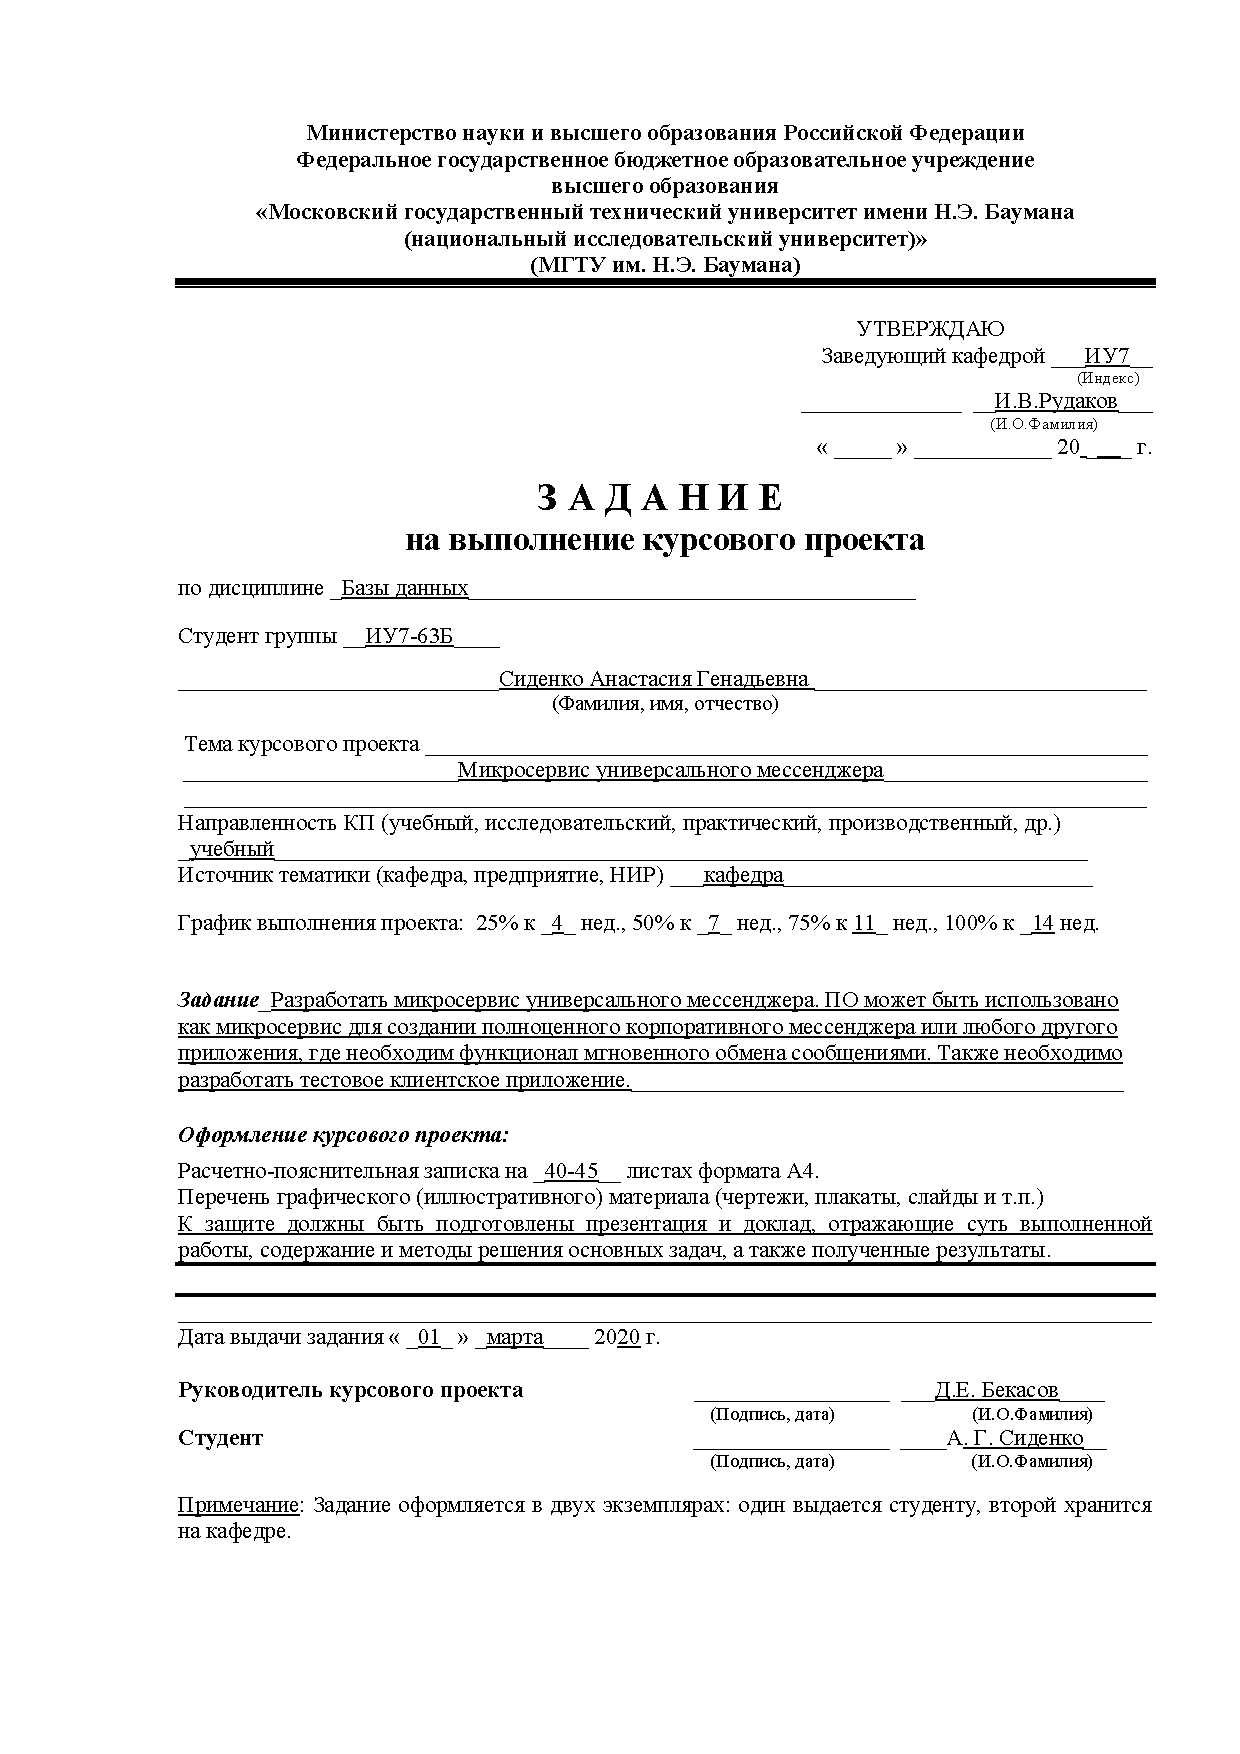
\includepdf[pages=-]{image/tz.pdf}

\frontmatter % выключает нумерацию ВСЕГО; здесь начинаются ненумерованные главы: реферат, введение, глоссарий, сокращения и прочее.

% Также можно использовать \Referat, как в оригинале
\Referat

\hfill

Курсовой проект представляет собой микросервис уни­версального мессенджера.

Ключевые слова: микросервис, мессенджер, универсальный, PostreSQL, ASP.NET Core, Entity Framework Core, REST. 

Данный микросервис реализуется на языке программирования C$\#$  с­ использованием платформы ASP.NET Core и технологии Entity Framework Core. Для взаимодействия между клиентом и сервером используется архитектурный стиль REST.

Полученное в результате работы ПО может быть использовано как микросервис для создании полноценного корпоративного мессенджера или любого другого приложения, где необходим функционал мгновенного обмена сообщениями. 

Отчёт содержит \pageref{LastPage}\,~страниц%
    \ifnum \totfig >0
    , \totfig~рисунка%
    \fi
    \ifnum \tottab >0
    , \tottab~таблицы%
    \fi
    %
    \ifnum \totbib >0
    , \totbib~источников%
    \fi
    %
    \ifnum \totapp >0
    , \totapp~прил.%
    \else
    .%
    \fi

%%% Local Variables: 
%%% mode: latex
%%% TeX-master: "rpz"
%%% End: 


\tableofcontents
%\printnomenclature % Автоматический список сокращений

\Introduction

\hfill

	На сегодняшний день более 4,5 миллиарда людей пользуются интернетом, а аудитория социальных сетей перевалила за отметку в 3,8 миллиарда \cite{useinternet}.
	
	Получается, что общение посредством мессенджеров является неотъемлемой частью жизни современного человека. 
	
	Практически все компании сталкиваются с вопросом: <<Какой использовать корпоративный мессенджер?>>. Он должен объединять все внутренние и внешние коммуникации в одно пространство. Сегодня рынок корпоративных мессенджеров предлагает десятки вариантов с разным функционалом, интеграцией с другими сервисами и ценовой политикой. Такие как, Slack, Microsoft Teams, Тwist, Discord и другие \cite{corporatemessengers}. 
	
	Однако данные приложения имеют ряд недостатков:
	\begin{itemize}
	\item сотрудники могут пользоваться различными мессенджерами;
	\item в контактах могут присутствовать люди, не имеющие отношения к работе, что служит отвлекающим фактором;
	\item недостаточная функциональность;
	\item безопасность. 
	\end{itemize}
	
	Для удобства коммуникации и работы внутри компании разрабатываются свои корпоративные внутренние средства общения, которые компенсируют вышеописанные недостатки. 
		
	Таким образом можно сделать вывод, что создание универсального мессенджера является актуальной темой, так как данное приложение будет ориентировано на специфику конкретной компании.
	
	Целью данной работы является реализация микросервиса универсального мессенджера.  Функциональное назначение микросервиса --- хранение и работа с данными.
	
	Для достижения поставленной цели необходимо решить следующие задачи. 
	\begin{enumerate}
		\item[1. ] Анализ существующих решений. 
		\item[2. ] Проектирование микросервиса мессенджера. 
		\item[3. ] Реализация микросервиса. 
		\item[4. ] Разработка тестового клиентского приложения. 
	\end{enumerate}





\mainmatter % это включает нумерацию глав и секций в документе ниже

\chapter{\textbf{Аналитический раздел}}
\hfill

Целью работы является создание микросервиса для универсального корпоративного мессенджера. В данном разделе рассматриваются существующие решения, производится выбор СУБД. 

\section{\textbf{Постановка задачи}}

Требуется разработать микросервис универсального корпоративного мессенджера, который обладает следующей функциональностью:
\begin{itemize}
\item создание, удаление, изменение параметров пользователей, хранение истории изменений;
\item создание, удаление, изменение параметров чата, хранение истории изменений;
\item добавление, удаление, изменение параметров участников чата, хранение истории изменений;
\item отправка сообщений, файлов, хранение истории изменений;
\item возможность добавления сообщения в избранное, закрепление сообщений в чатах, хранение истории изменений. 
\end{itemize}

Система должна иметь интерфейс для демонстрации работы микросервиса. Микросервис осуществляет работу с базой данных, обрабатывает и обслуживает запросы пользователей. 

\section{\textbf{Обзор и анализ существующих решений, обоснование необходимости разработки}}

В настоящее время существует большое число различных корпоративных мессенджеров, которые решают вопрос коммуникации сотрудников внутри компании, а также поддерживает связь с клиентами, подрядчиками и партнерами  \cite{comandmessenger}.

\subsection{\textbf{Slack}}

Slack \cite{slack} -- первый корпоративный мессенджер, предложил решение, позволяющее избавиться от многочисленных писем в почте и структуризировать коммуникацию внутри команды. Далее разбивается на отдельные каналы по проектам или отделам. Имеет огромный функционал. 

В бесплатной версии Slack поддерживает неограниченное число пользователей, интеграцию с 10 внешними сервисами и поиск в архиве до 10 тысяч сообщений. В платных тарифах -- 6,67\$ (Standard) и 12,5\$ (Plus) за пользователя в месяц -- снимаются ограничения и появляются дополнительные возможности для управления правами доступа. 

На рисунке \ref{img:slack} показан интерфейс мессенджера Slack. 

\begin{figure}[H]
	\centering
	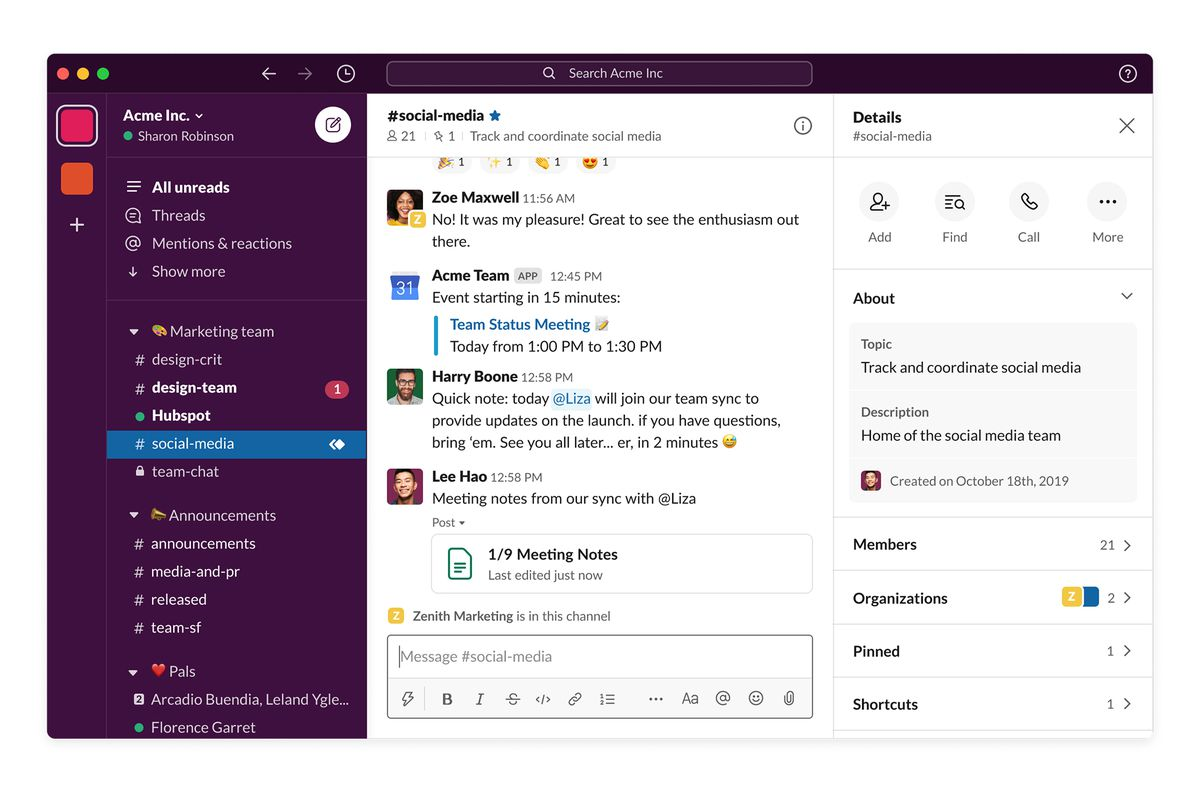
\includegraphics[scale=0.4]{slack}
	\caption{Интерфейс Slack. }
	\label{img:slack}
\end{figure}

\subsection{\textbf{Microsoft Teams}}

Microsoft Teams \cite{micteams} является альтернативой Slack. Возможность создания команд, общения посредством чата. Удобная интеграция со всеми сервисами Office 365. Однако, по сравнению со Slack, всего около 200 внешних сервисов (в Slack порядка тысячи). 

Ценовая политика лояльнее. Так, в бесплатный план входит неограниченная история сообщений, конференции до 250 человек, совместное использование экрана. Самый доступный платный план для Microsoft Teams -- \$ 5 с пользователя в месяц. 

На рисунке \ref{img:microsoftteams} показан интерфейс мессенджера Microsoft Teams. 

\begin{figure}[H]
	\centering
	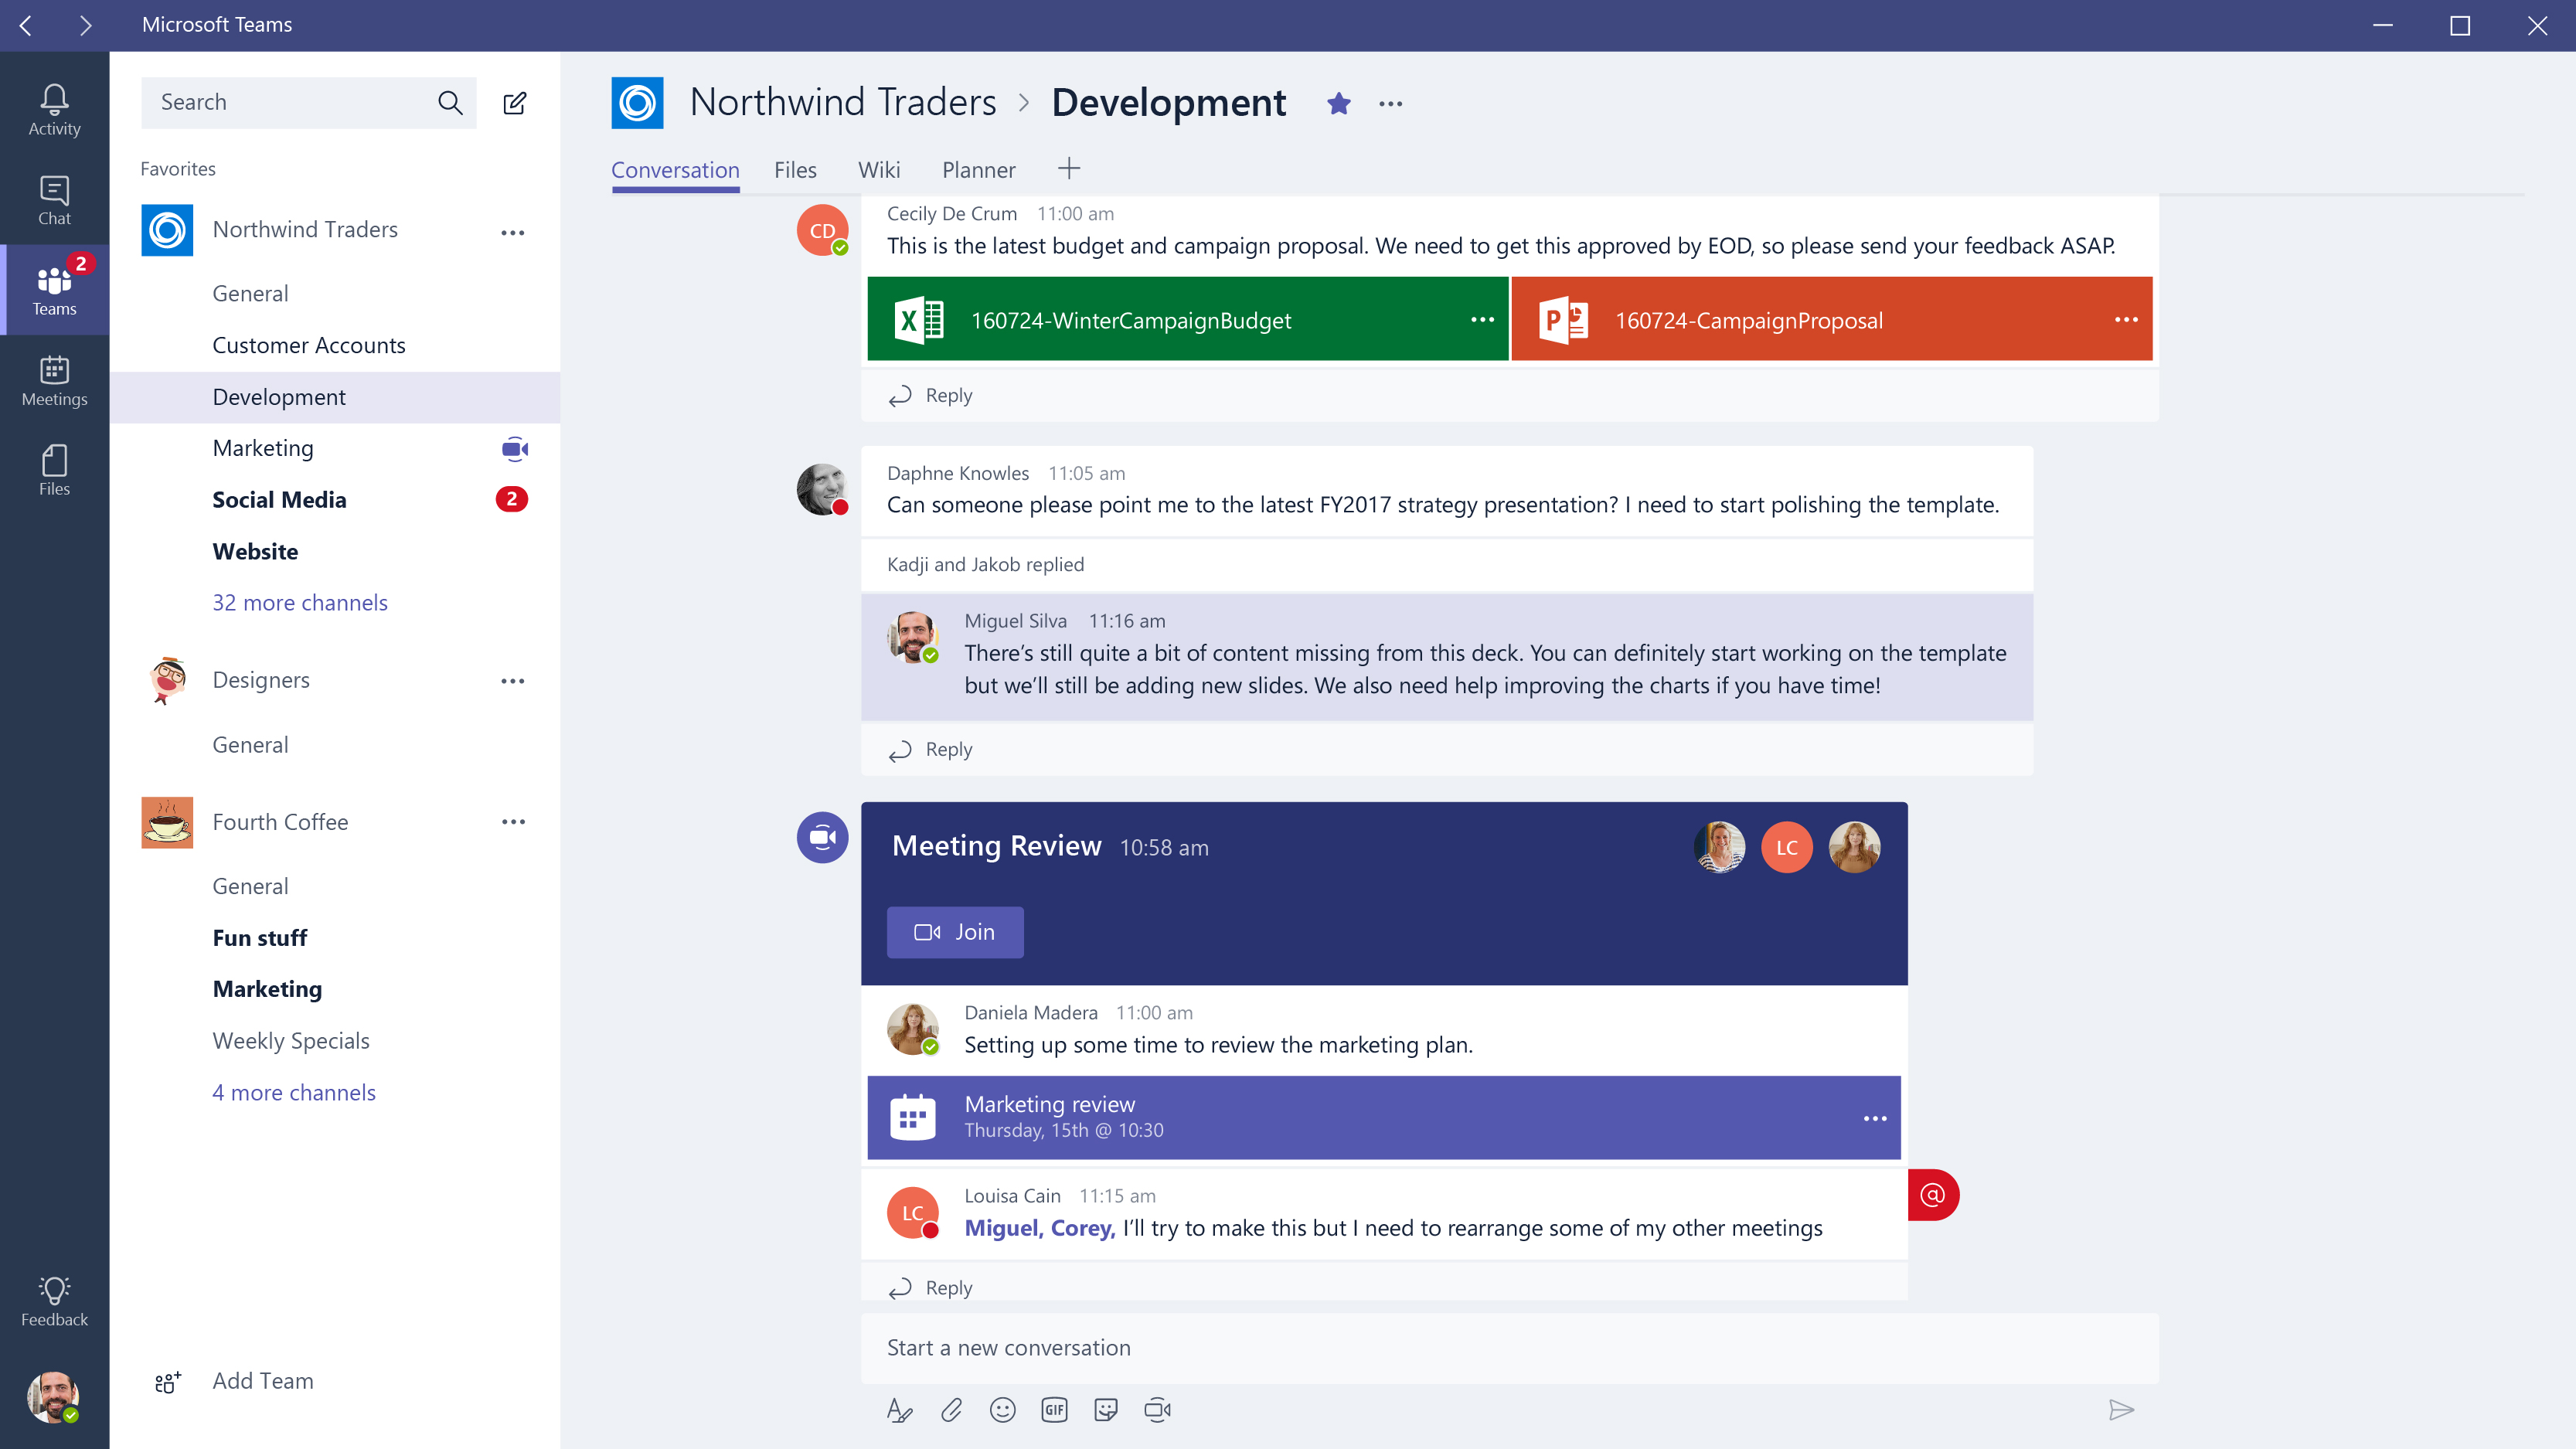
\includegraphics[scale=0.3]{microsoftteams}
	\caption{Интерфейс Microsoft Teams. }
	\label{img:microsoftteams}
\end{figure}

\subsection{\textbf{Twist}}

Twist \cite{twist} -- это успешная альтернатива Slack. Основное отличие в том, чтобы больше времени работать, и меньше отвлекаться на постоянные уведомления и чаты. Работа в мессенджере построена по принципу обсуждений -- для каждой задачи создаётся отдельный чат, в который можно пригласить членов команды. Обсуждения можно разделить по каналам -- в соответствии с общей темой. Таким образом, нет необходимости долго искать нужное обсуждение. 

Как и Slack, использование мессенджера бесплатно для команд, которым не нужен доступ к полной истории сообщений. Для остальных стоимость составит 329 $\rouble$ в месяц за человека.

На рисунке \ref{img:twist} показан интерфейс мессенджера Twist. 

\begin{figure}[H]
	\centering
	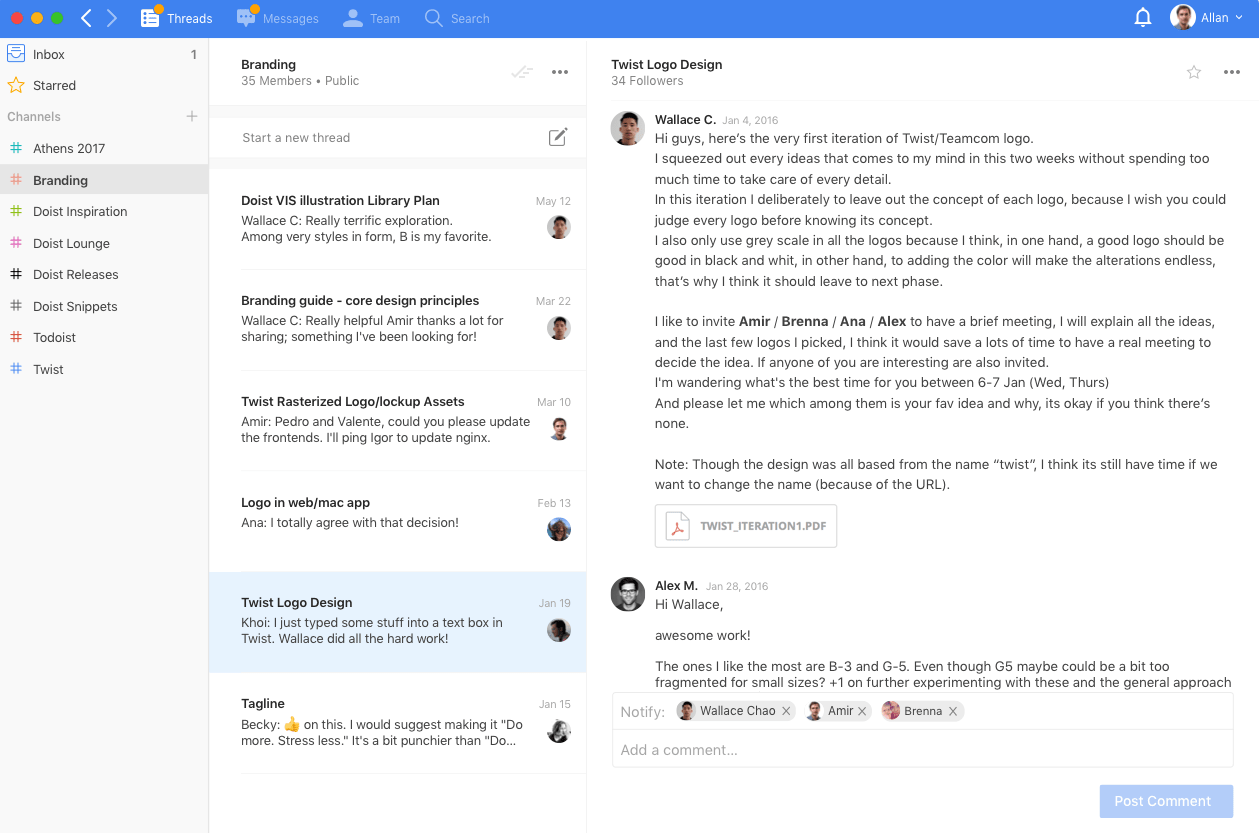
\includegraphics[scale=0.35]{twist}
	\caption{Интерфейс Twist. }
	\label{img:twist}
\end{figure}

\subsection{\textbf{Discord}}

Discord \cite{discord} -- игровой мессенджер. У пользователя в нём есть свой аккаунт, через который он может общаться с друзьями из списка контактов, а может присоединится к неограниченному количеству команд. Команды создаются бесплатно и в них также может быть неограниченное количество участников. Внутри всё устроено наподобие Slack: есть каналы, есть приватные каналы, есть возможность общаться напрямую. 

На рисунке \ref{img:discord} показан интерфейс мессенджера Discord. 

\begin{figure}[H]
	\centering
	\includegraphics[scale=0.4]{discord}
	\caption{Интерфейс Discord. }
	\label{img:discord}
\end{figure}

\subsection{\textbf{Rocket.Chat}}

Rocket.Chat \cite{rocket} --- это мессенджер с открытым исходным кодом, который поддерживает групповые чаты, обмен файлами, видеоконференции, ботов и многое другое. Rocket.Chat можно также установить на собственный сервер, а затем общаться, используя веб-интерфейс, персональный компьютер или мобильное устройство. Или использовать платную версию для облачного хранения. 

Можно добавлять новую функциональность. 

На рисунке \ref{img:rocket} показан интерфейс мессенджера Rocket.Chat. 

\begin{figure}[H]
	\centering
	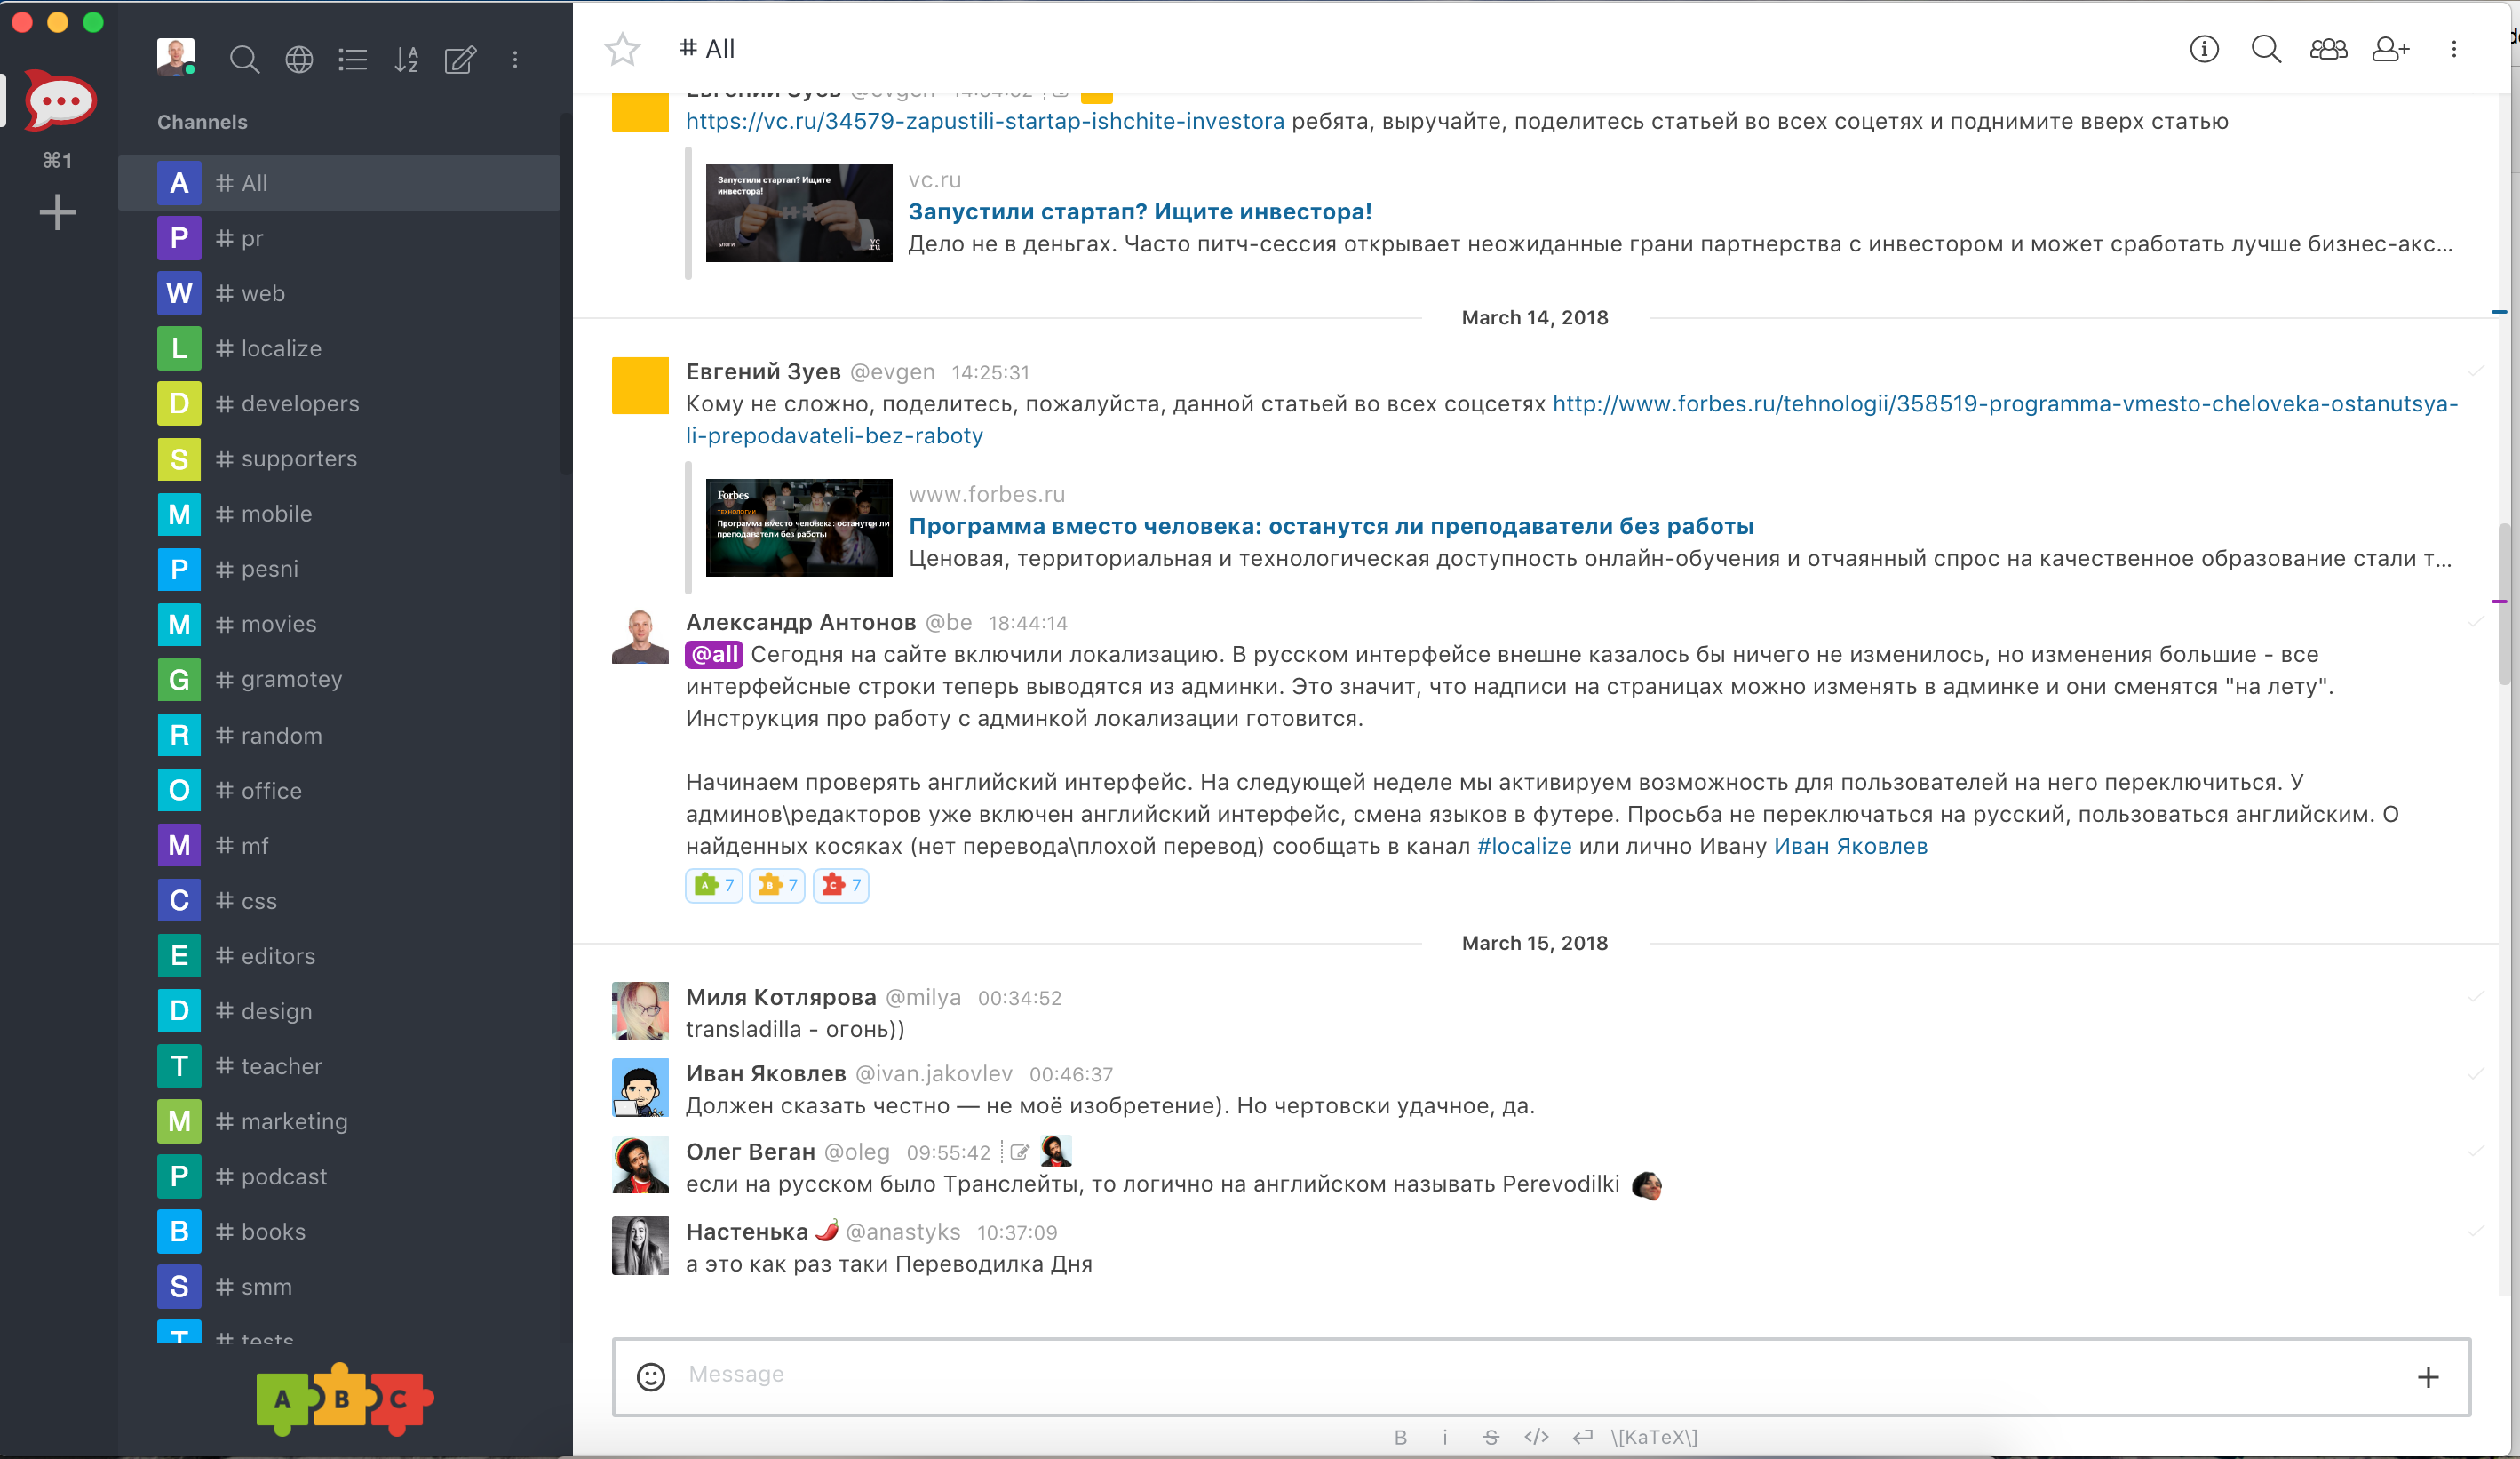
\includegraphics[scale=0.17]{rocket}
	\caption{Интерфейс Rocket.Chat. }
	\label{img:rocket}
\end{figure}


На основе аналогов и поставленных цели и задач можно выделить следующие критерии сравнения:

\begin{itemize}
\item создание обсуждения задач;
\item несколько закрепленных сообщения;
\item избранные сообщения для отдельных пользователей;
\item хранение всей истории изменений (чаты, сообщения, пользователи);
\item разные имена пользователей в различных чатах;
\item наличие различных прав у пользователей; 
\item возможность хранения на собственном сервере. 
\end{itemize}

В таблице \ref{table:messagecompare} представлено сравнение мессенджеров по вышепредставленным параметрам. 

\begin{table}[H]
\caption{Сравнение мессенджеров. }
\begin{tabular}{|p{5cm}|p{1.9cm}|p{1.9cm}|p{1.9cm}|p{1.9cm}|p{1.5cm}|}
\hline
 & Slack & Microsoft Teams  & Twist & Discord & Rocket. Chat  \\ \hline
Создание обсуждения задач & + (прям в чате) & + & + & - & - \\ \hline
Несколько закрепленных сообщения & +  & - & - &  + (ограничение 50)  & +  \\ \hline
Избранные сообщения для отдельных пользователей  & +  & - & - & -  & + \\ \hline
Хранение всей истории изменений (чаты, сообщения, пользователи)& - &-& - & - & - \\ \hline
Разные имена пользователей в различных чатах& - & +& - &  + & + \\ \hline
Наличие различных прав у пользователей& - & + & + &  + & + \\ \hline
Возможность хранения на собственном сервере& - & - & - &  - & + \\ \hline
\end{tabular}
\label{table:messagecompare}
\end{table}

\textbf{Актуальность темы} обусловлена отсутствием универсального мессенджера с полной историей изменения чатов, пользователей, сообщений. А ещё у рассмотренных готовых решений вся переписка хранится на облачных серверах мессенджера. Данный факт не устраивает большое количество компаний, которым желательно хранить все данные на своих серверах. 

\section{\textbf{Анализ типов и выбор СУБД}}

Цели и задачи поставлены необходимо определиться с СУБД. 

\subsection{\textbf{Типы СУБД}}

Системы управления базами данных (СУБД) -- это высокоуровневое программное обеспечение, работающее с низкоуровневыми API. Для решения проблем создавались различные виды СУБД. Два основных направления -- реляционные (SQL) и нереляционные (NoSQL) СУБД \cite{nosql}. СУБД основаны на моделях баз данных. 

\subsubsection{\textbf{Реляционная модель}}

Представленная в 70-х, реляционная модель предлагает структурированное хранение данных. Отношения дают возможность группировки данных как связанных наборов, представленных в виде таблиц, содержащих упорядоченную информацию и соотносящих значения и атрибуты. РСУБД работают производительно и надёжно. Несмотря на строгие принципы формирования и обработки данных, РСУБД могут быть гибкими.

\subsubsection{\textbf{Иные подходы}}

NoSQL-способ структуризации данных заключается в избавлении от ограничений при хранении и использовании информации. Базы данных NoSQL, используя неструктуризированный подход, предлагают много эффективных способов обработки данных в отдельных случаях. 

В таблице \ref{table:subd} представлено сравнение 2 этих подходов. 

\begin{table}[H]
\caption{Сравнение моделей БД. }
\begin{tabular}{|p{5cm}|p{5cm}|p{5cm}|}
\hline
 & SQL & NoSQL  \\ \hline
Структура и тип хранящихся данных & Однозначно определёная структура хранения данных & Ограничений нет \\ \hline
Запросы & Получение данных при помощи языка SQL&  Каждая NoSQL база данных реализует свой способ работы с данными \\ \hline
Масштабируемость  & Не подходит для постоянно меняющихся структур данных & Подходит для постоянно меняющихся структур данных \\ \hline
Поддержка & Развитая СУБД, наличие большого сообщества вокруг неё, множество примеров & Только недавно стала популярной \\ \hline
Объединение таблиц & Применени join & Отсутствие join \\ \hline
\end{tabular}
\label{table:subd}
\end{table}

Так как, данные имеют четкую структуру и заранее определены, выбор в пользу реляционной базы данных. 

\subsection{\textbf{Выбор реляционной СУБД}}

Одними из самых популярных РСУБД сейчас являются MSSQL, MySQL, PostgreSQL, Oracle.

\subsubsection{\textbf{MSSQL}}

Microsoft SQL Server -- разработанная корпорацией майкрософт, система управления реляционными базами данных.

Преимущества
\begin{itemize}
\item простота: MSSQL легко устанавливается и используется;
\item возможность регулировки и отслеживания уровня производительности, чтобы уменьшить загрузку;
\item возможность интеграции с другими продуктами Microsoft;
\item визуализация на мобильных устройствах.
\end{itemize}

Недостатки
\begin{itemize}
\item высокая стоимость продукта для юридических лиц;
\item возможны проблемы в работе служб интеграции импорта файлов;
\item высокая ресурсоемкость SQL Server.
\end{itemize}

\subsubsection{\textbf{MySQL}}

MySQL -- это самая популярная из всех крупных серверных БД. Разобраться в ней просто, большое количество информации. 

Преимущества
\begin{itemize}
\item простота: MySQL легко устанавливается и используется;
\item много функций: MySQL поддерживает большую часть функционала SQL;
\item безопасность: в MySQL встроено много функций безопасности;
\item мощность и масштабируемость: MySQL может работать с действительно большими объёмами данных, и неплохо походит для масштабируемых приложений;
\item скорость: пренебрежение некоторыми стандартами позволяет MySQL работать производительнее.
\end{itemize}

Недостатки
\begin{itemize}
\item ограничения функциональности, так как не полностью реализованы SQL-стандарты;
\item надёжность: некоторые операции реализованы менее надёжно, чем в других РСУБД;
\item застой в разработке: хотя MySQL и является open-source продуктом, работа над ней сильно заторможена.
\end{itemize}

\subsubsection{\textbf{PostgreSQL}}

PostgreSQL -- это РСУБД, ориентирующаяся в первую очередь на полное соответствие стандартам и расширяемость.

Преимущества
\begin{itemize}
\item полная SQL-совместимость;
\item cообщество: PostgreSQL поддерживается опытным сообществом 24/7;
\item поддержка сторонними организациями;
\item расширяемость: PostgreSQL можно программно расширить за счёт хранимых процедур. 
\end{itemize}

Недостатки
\begin{itemize}
\item производительность: в простых операциях чтения PostgreSQL может уступать своим аналогам. 
\end{itemize}

\subsubsection{\textbf{Oracle}}

Oracle -- это объектно-реляционная система управления базами данных.

Преимущества
\begin{itemize}
\item поддержка огромных баз данных и большого числа пользователей;
\item быстрая обработка транзакций;
\item большой и постоянно развивающийся функционал. 
\end{itemize}

Недостатки
\begin{itemize}
\item высокая стоимость;
\item требуются значительные вычислительные ресурсы.  
\end{itemize}

PostgreSQL выигрывает по многим параметрам и бесплатно распространяется. Поэтому было принято решение использовать именно эту РСУБД.

\section{\textbf{Вывод}}

В данном разделе были рассмотрены существующие решения, была выбрана СУБД и поставлена задача реализации микросервиса мессенджера с хранением истории, возможностью добавлять сообщения в избранное и закреплять в чатах. 
\chapter{\textbf{Конструкторский раздел}}

\hfill

Можно разбить задачу проектирования микросервиса на подзадачи:
\begin{itemize}
\item описание функциональности и поведения;
\item выделение сущностей предметной области;
\item разработка структуры БД;
\item проектирование компонентов микросервиса.
\end{itemize}

В данном раздел рассматривается структура микросервиса мессенджера, каждого из его компонентов. 

\section{\textbf{Функциональная модель}}

\hfill

На рисунке \ref{img:idef0} изображена функциональная модель, отобра­жающая структуру и функции системы.

\begin{figure}[H]
	\centering
	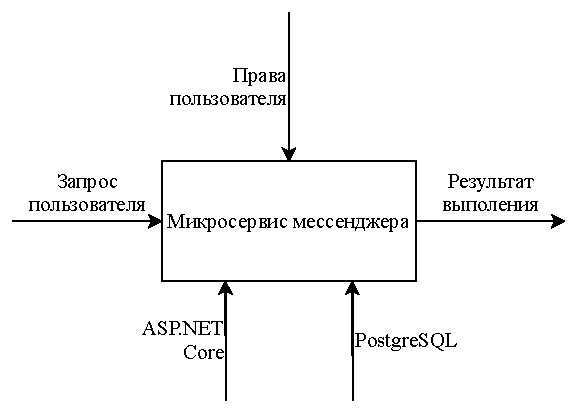
\includegraphics[scale=1]{idef0}
	\caption{Функциональная модель микросервиса мессенджера. }
	\label{img:idef0}
\end{figure}

\section{\textbf{Сценарий использования}}

\hfill

В данном разделе необходимо построить Use Case Diagram (диаграмму прецедентов). Она состоит из графической диаграммы, описывающей действующие лица и прецеденты -- конкретные действия, которые выполняет пользователь при работе с системой. 

Данная диаграмма предназначена для определения функциональных требований, действующие лица не будут делится по ролям и правам, так как за это отвечает внешняя система. 

На рисунке \ref{img:usechat} представлена Use Case диаграмма для действий с чатами. 

\begin{figure}[H]
	\centering
	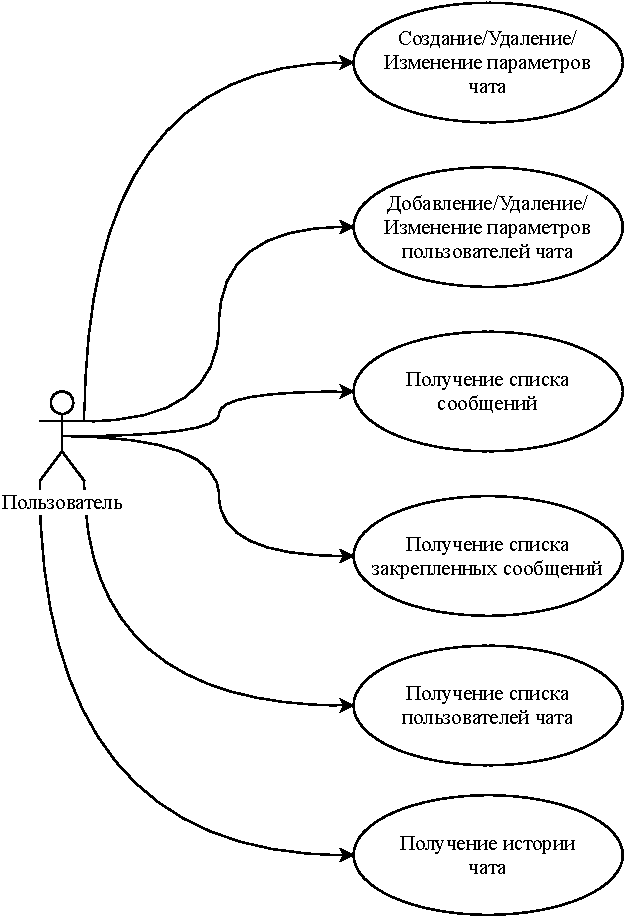
\includegraphics[scale=1]{usechat}
	\caption{Use Case диаграмма для действий с чатами. }
	\label{img:usechat}
\end{figure}

На рисунке \ref{img:useuser} представлена Use Case диаграмма для действий с пользователями. 

\begin{figure}[H]
	\centering
	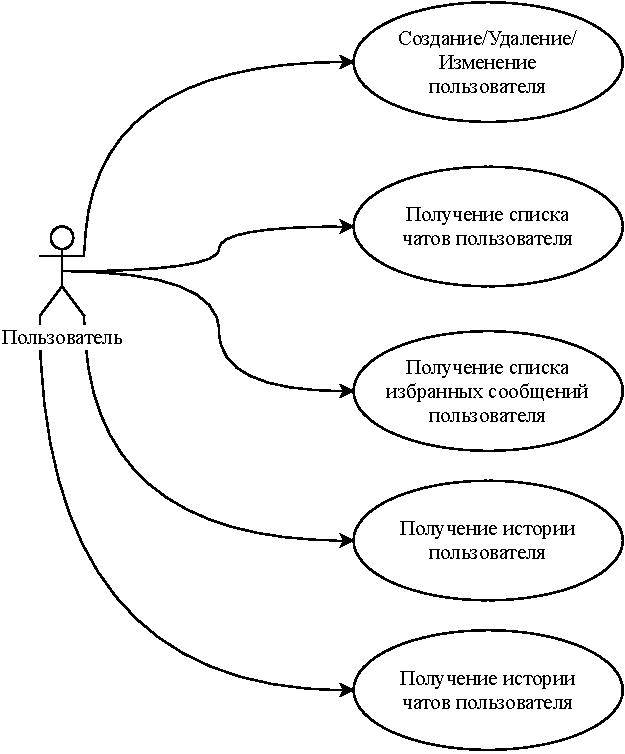
\includegraphics[scale=1]{useuser}
	\caption{Use Case диаграмма для действий с пользователями. }
	\label{img:useuser}
\end{figure}

На рисунке \ref{img:usemessage} представлена Use Case диаграмма для действий с сообщениями. 

\begin{figure}[H]
	\centering
	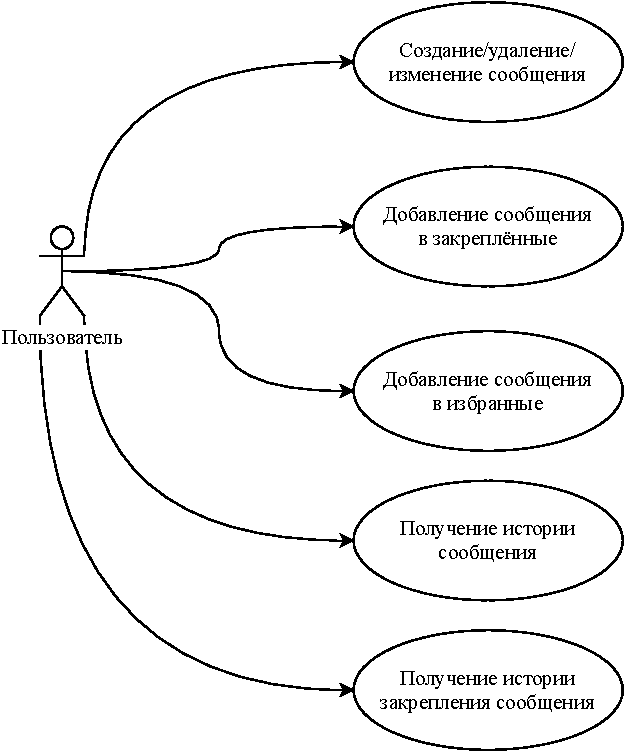
\includegraphics[scale=1]{usemessage}
	\caption{Use Case диаграмма для действий с сообщениями. }
	\label{img:usemessage}
\end{figure}


\section{\textbf{База данных}}

\hfill

Далее были выделены сущности предметной области и построена ER-диаграмма, которая содержит 14 таблиц. Диаграмма представлена на рисунке \ref{img:er}. Таблица \ref{table:database} содержит описание сущностей базы данных. 

\begin{figure}[H]
	\centering
	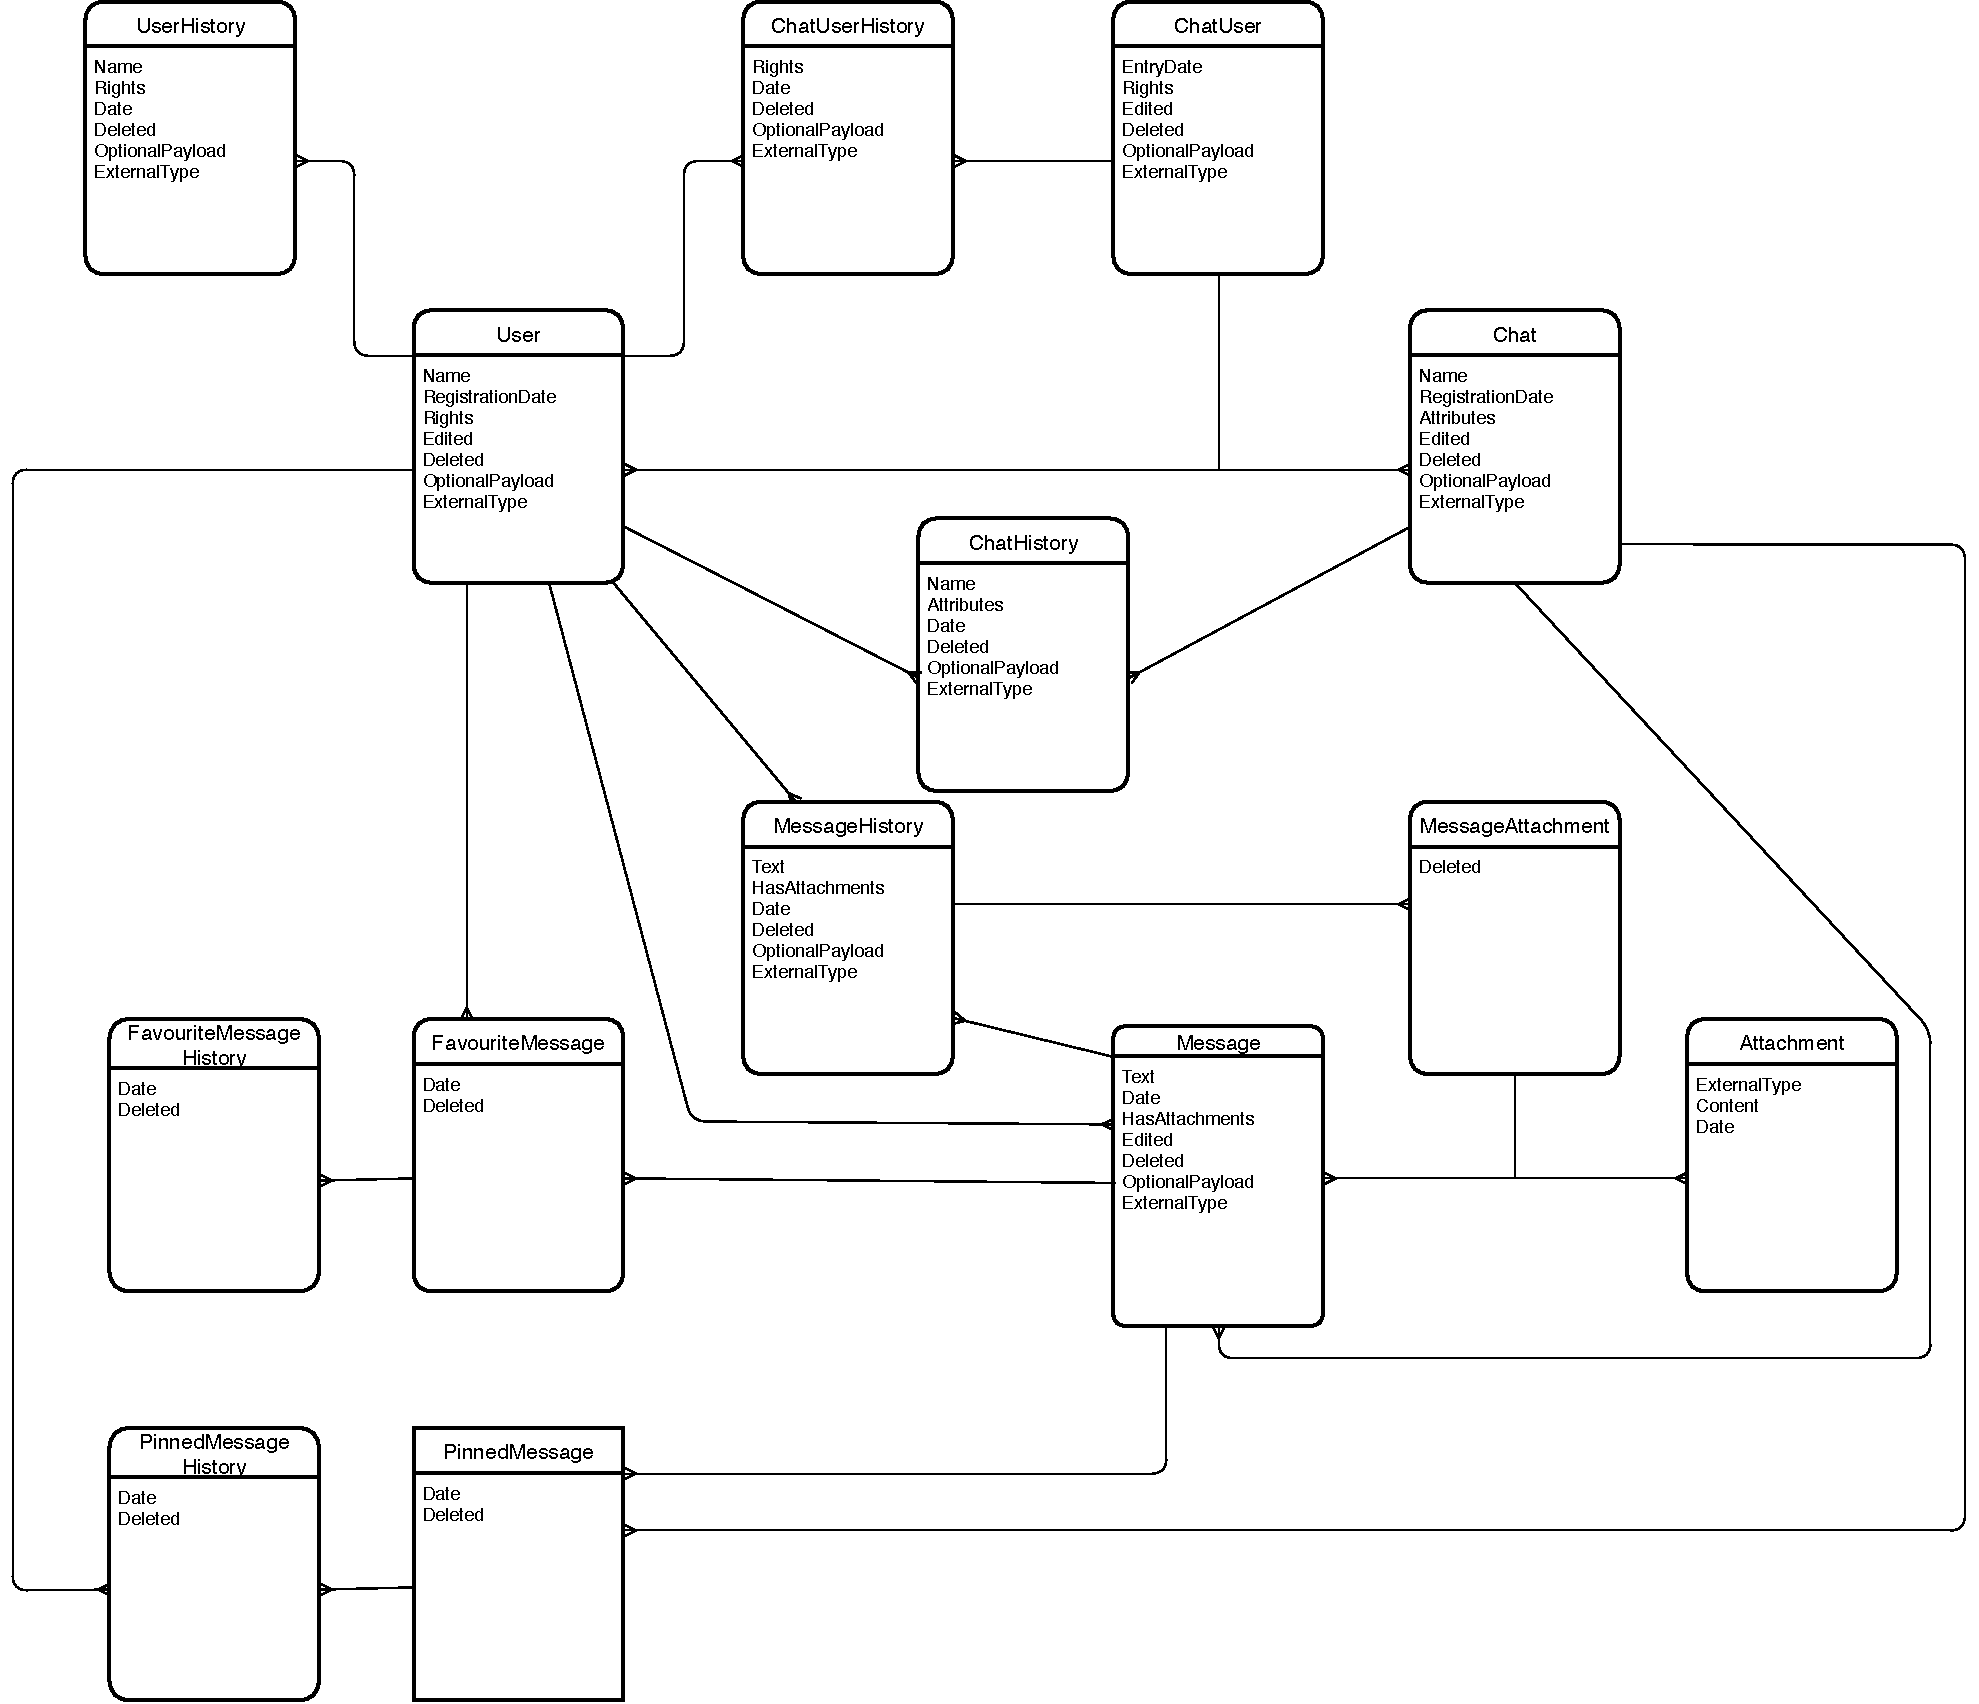
\includegraphics[scale=0.53]{er}
	\caption{ER-диаграмма базы данных. }
	\label{img:er}
\end{figure}

\begin{table}[H]
\caption{Описание сущностей базы данных. }
\begin{tabular}{|p{4cm}|p{12cm}|}
\hline
Название таблицы&Описание \\ \hline
User & Пользователи \\ \hline
UserHistory & История изменений пользователей \\ \hline
Chat & Чаты \\ \hline
ChatHistory & История изменений чатов \\ \hline
ChatUser & Пользователи чатов (соединительная таблица между пользователями и чатами) \\ \hline
ChatUserHistory & История изменений пользователей чата \\ \hline
Message & Сообщения \\ \hline
MessageHistory & История изменений сообщений \\ \hline
Attachment & Вложения \\ \hline
MessageAttachment & Вложения сообщений (соединительная таблица между вложениями и сообщениями)  \\ \hline
FavouriteMessage & Избранные сообщения пользователя \\ \hline
FavouriteMessage History & История изменений избранных сообщений пользователя \\ \hline
PinnedMessage & Закрепленные сообщения в чатах \\ \hline
PinnedMessage History & История изменений закрепленных сообщений в чатах \\ \hline
\end{tabular}
\label{table:database}
\end{table}

\section{\textbf{Проектирование архитектуры}}

\hfill

Необходимо спроектировать абстрактный микросервис мессенджера. На рисунке \ref{img:components} представлена диаграмма компонентов микросервиса. 

\begin{figure}[H]
	\centering
	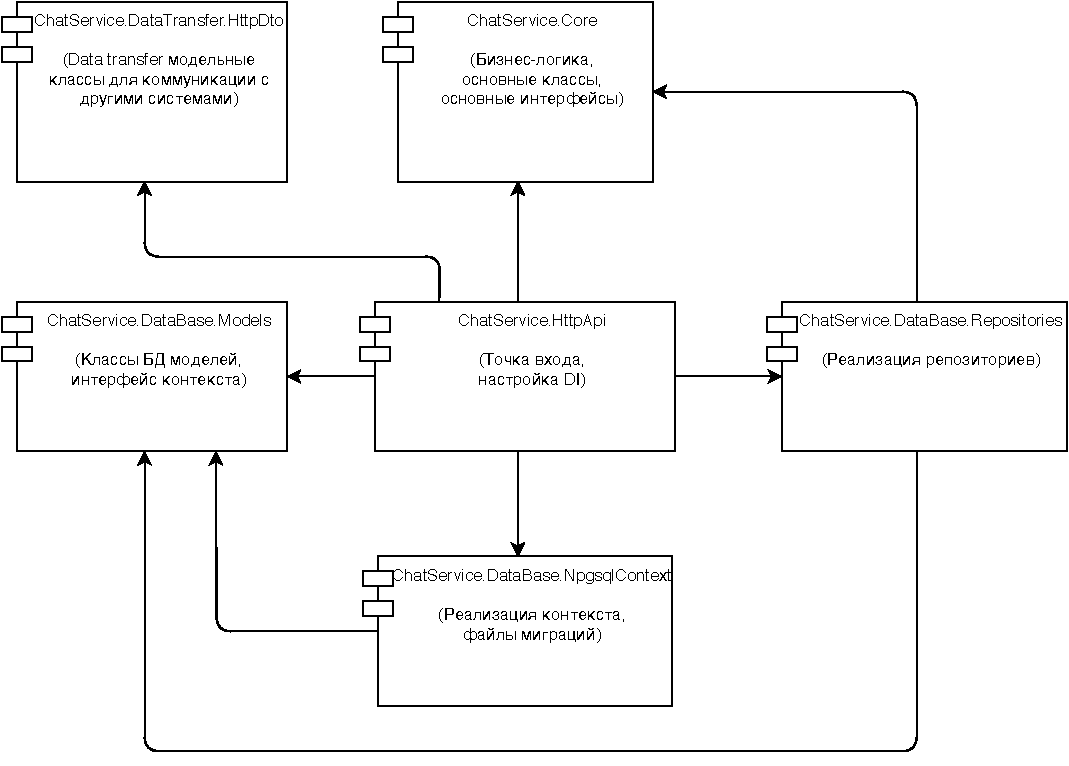
\includegraphics[scale=0.95]{components}
	\caption{Диаграмма компонентов микросервиса. }
	\label{img:components}
\end{figure}

\begin{enumerate}
\item[1. ] \textbf{ChatService.HttpApi}

ChatService.HttpApi -- точка входа в проект, инициализирует и конфигурирует IoC контейнер, здесь происходит настройка DI. 

Смысл IoC (Inversion of Control/инверсия управления) заключается в том, что модули верхнего уровня не должны зависеть от реализации модулей нижнего уровня \cite{solid}. То есть, например, компонент в приложении, который отвечает за модели базы данных, не должен зависеть от конкретной используемой СУБД. Вместо этого передается интерфейс.

IoC контейнер знает о всех интерфейсах и их реализациях в системе и умеет их сопоставлять. Делается это через DI. 

DI (Dependency Injection/внедрение зависимостей) -- это процесс предоставления внешней зависимости программному компоненту. Перед началом работы с контейнером необходимо зарегистрировать известные типы и их сопоставления (интерфейс $\longrightarrow$ реализация).

\item[2. ] \textbf{ChatService.Database.Models}

В компоненте ChatService.Database.Models описываются классы сущностей базы данных из рисунка \ref{img:er} и интерфейс IChatServiceContext. 

\item[3. ] \textbf{ChatService.Database.NpgsqlContext}

ChatServiceContext -- класс, который позволяет взаимодействовать с базой данных используя сущностную модель классов. Класс контекста позволяет вам создавать и выполнять запросы, отслеживать изменения в объектах и отображать эти изменения на базу данных

\item[4. ] \textbf{ChatService.Database.Repositories}

В ChatService.Database.Repositories описываются реализации репозиториев. 

Паттерн Репозиторий позволяет абстрагироваться от конкретных подключений к источникам данных, с которыми работает программа, и является промежуточным слоем между классами, непосредственно взаимодействующими с данными, и основными классами программы.

Преимущества использования данного паттерна:
\begin{itemize}
\item разделение логики (обращаемся только к тем данным, которые нужны);
\item абстрагирование от способа хранения данных;
\item легкость тестирования (можно передавать заглушку репозитория при тестировании бизнес-логики). Конкретная реализация репозитория регистрируется в IoC. 
\end{itemize}

\item[5. ] \textbf{ChatService.Core}

ChatService.Core -- компонент, содержащий всю бизнес-логику микросервиса мессенджера. Также, в него включены интерфейсы репозиториев и собственные модельные классы. 

Функциональность данного класса:
\begin{itemize}
\item создание, удаление, изменение параметров пользователей;
\item создание, удаление, изменение параметров чата;
\item добавление, удаление, изменение параметров участников чата;
\item отправка сообщений, файлов;
\item возможность добавления сообщения в избранное, закрепление сообщений в чатах;
\item получение различной доступной информации.  
\end{itemize}

\item[6. ] \textbf{ChatService.DataTransfer.HttpDto}

ChatService.DataTransfer.HttpDto -- компонент используется для передачи данных между различными приложениями (в данном случае между микросервисом мессенджера и, например, клиентом). Это паттерн Data Transfer Object, который может хранить всю необходимую для вызова информацию. Он должен быть сериализуемым для удобной передачи по сети.

\end{enumerate}

\section{\textbf{Вывод}}

\hfill

Структура микросервиса мессенджера разработана, переход к реализации. 

\chapter{\textbf{Технологический раздел}}

\hfill

В соответствии с выбранной задачей -- реализация микросервиса мессенджера. Необходимо выбрать средства реализации, создать модули и интерфейс, описать ограничения и порядок работы программы. 

\section{\textbf{Выбор технологий}}

Для выполнения проекта был выбран язык программирования C$\#$ \cite{csharp}. Язык является постоянно развивающимся, объектно-ориентированным. Он относится к семье языков с C-подобным синтаксисом, разрабатывался как язык программирования прикладного уровня для CLR (Common Language Runtime, общеязыковая исполняющая среда). 

Для разработки используется платформа ASP.NET Core \cite{aspnet}, предназначенная для создания различного рода веб-приложений: от небольших веб-сайтов до крупных веб-порталов и веб-сервисов. С помощью ASP.NET Core мы можем создавать кросс-платформенные приложения. Благодаря модульности фреймворка все необходимые компоненты веб-приложения могут загружаться как отдельные модули через пакетный менеджер Nuget.

Для доступа к данным используется технология Entity Framework Core \cite{ef}. EF Core является ORM-инструментом (object-relational mapping -- отображения данных на реальные объекты). То есть EF Core позволяет работать базами данных, но представляет собой более высокий уровень абстракции: EF Core позволяет абстрагироваться от самой базы данных и ее таблиц и работать с данными независимо от типа хранилища. 

Entity Framework Core поддерживает множество различных систем баз данных. Таким образом, мы можем через EF Core работать с любой СУБД, если для нее имеется нужный провайдер. Для работы с PostgeSQL в проект необходимо добавить через Nuget пакет Npgsql.EntityFrameworkCore.PostgreSQL. 

Для взаимодействия между клиентом и сервером используется архитектурный стиль REST \cite{rest}. API-интерфейс может считаться RESTful только в том случае, если соблюдены все требования. При создании микросервиса мессенджера были учтены данные требования, и поэтому веб-приложение является RESTful. 

Требования REST:
\begin{itemize}
\item модель клиент-сервер;
\item отсутствие состояния (сервис не хранит информацию о состоянии клиента);
\item кэширование;
\item единообразие интерфейса (идентификация ресурсов, манипуляция ресурсами через представление, «самоописываемые» сообщения);
\item многослойность сервера;
\item код по требованию (необязательно). 
\end{itemize}

\section{\textbf{Модель базы данных}}

На рисунке \ref{img:database} представлена модель базы данных. 

\begin{figure}[H]
	\centering
	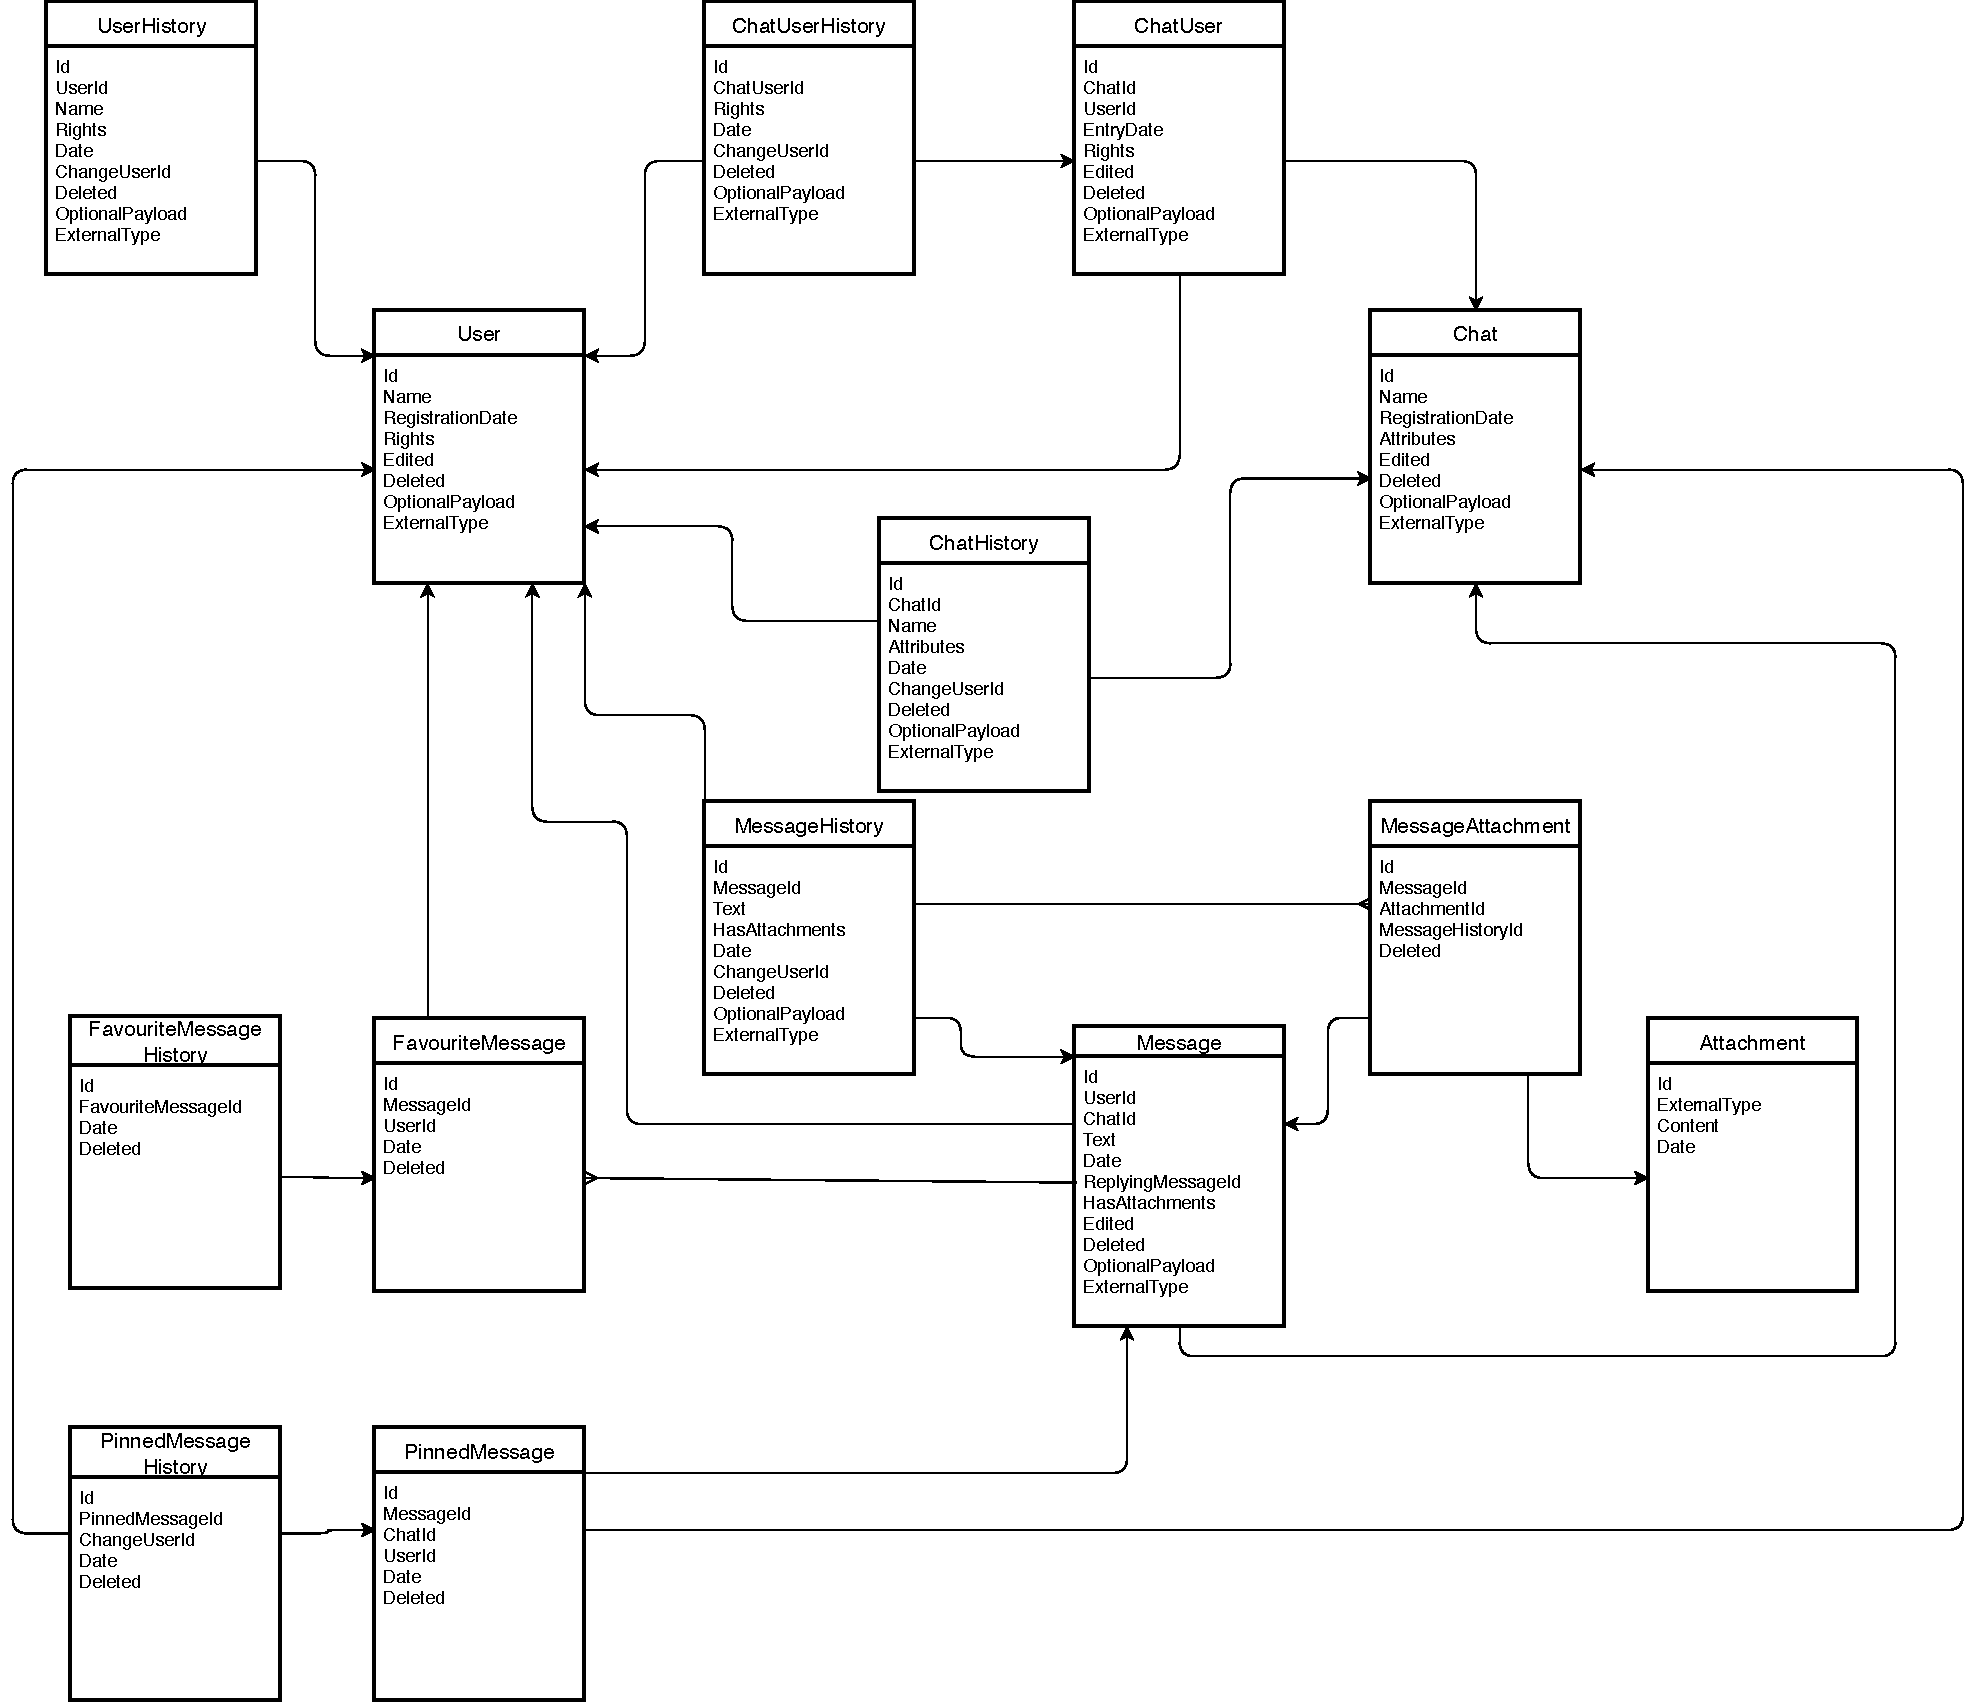
\includegraphics[scale=0.5]{database}
	\caption{Модель базы данных. }
	\label{img:database}
\end{figure}

\section{\textbf{UML-диаграммы классов }}

На рисунке \ref{img:databasemodels} представлена UML-диаграмма классов компонента ChatService.Database.Models. 

\begin{figure}[H]
	\centering
	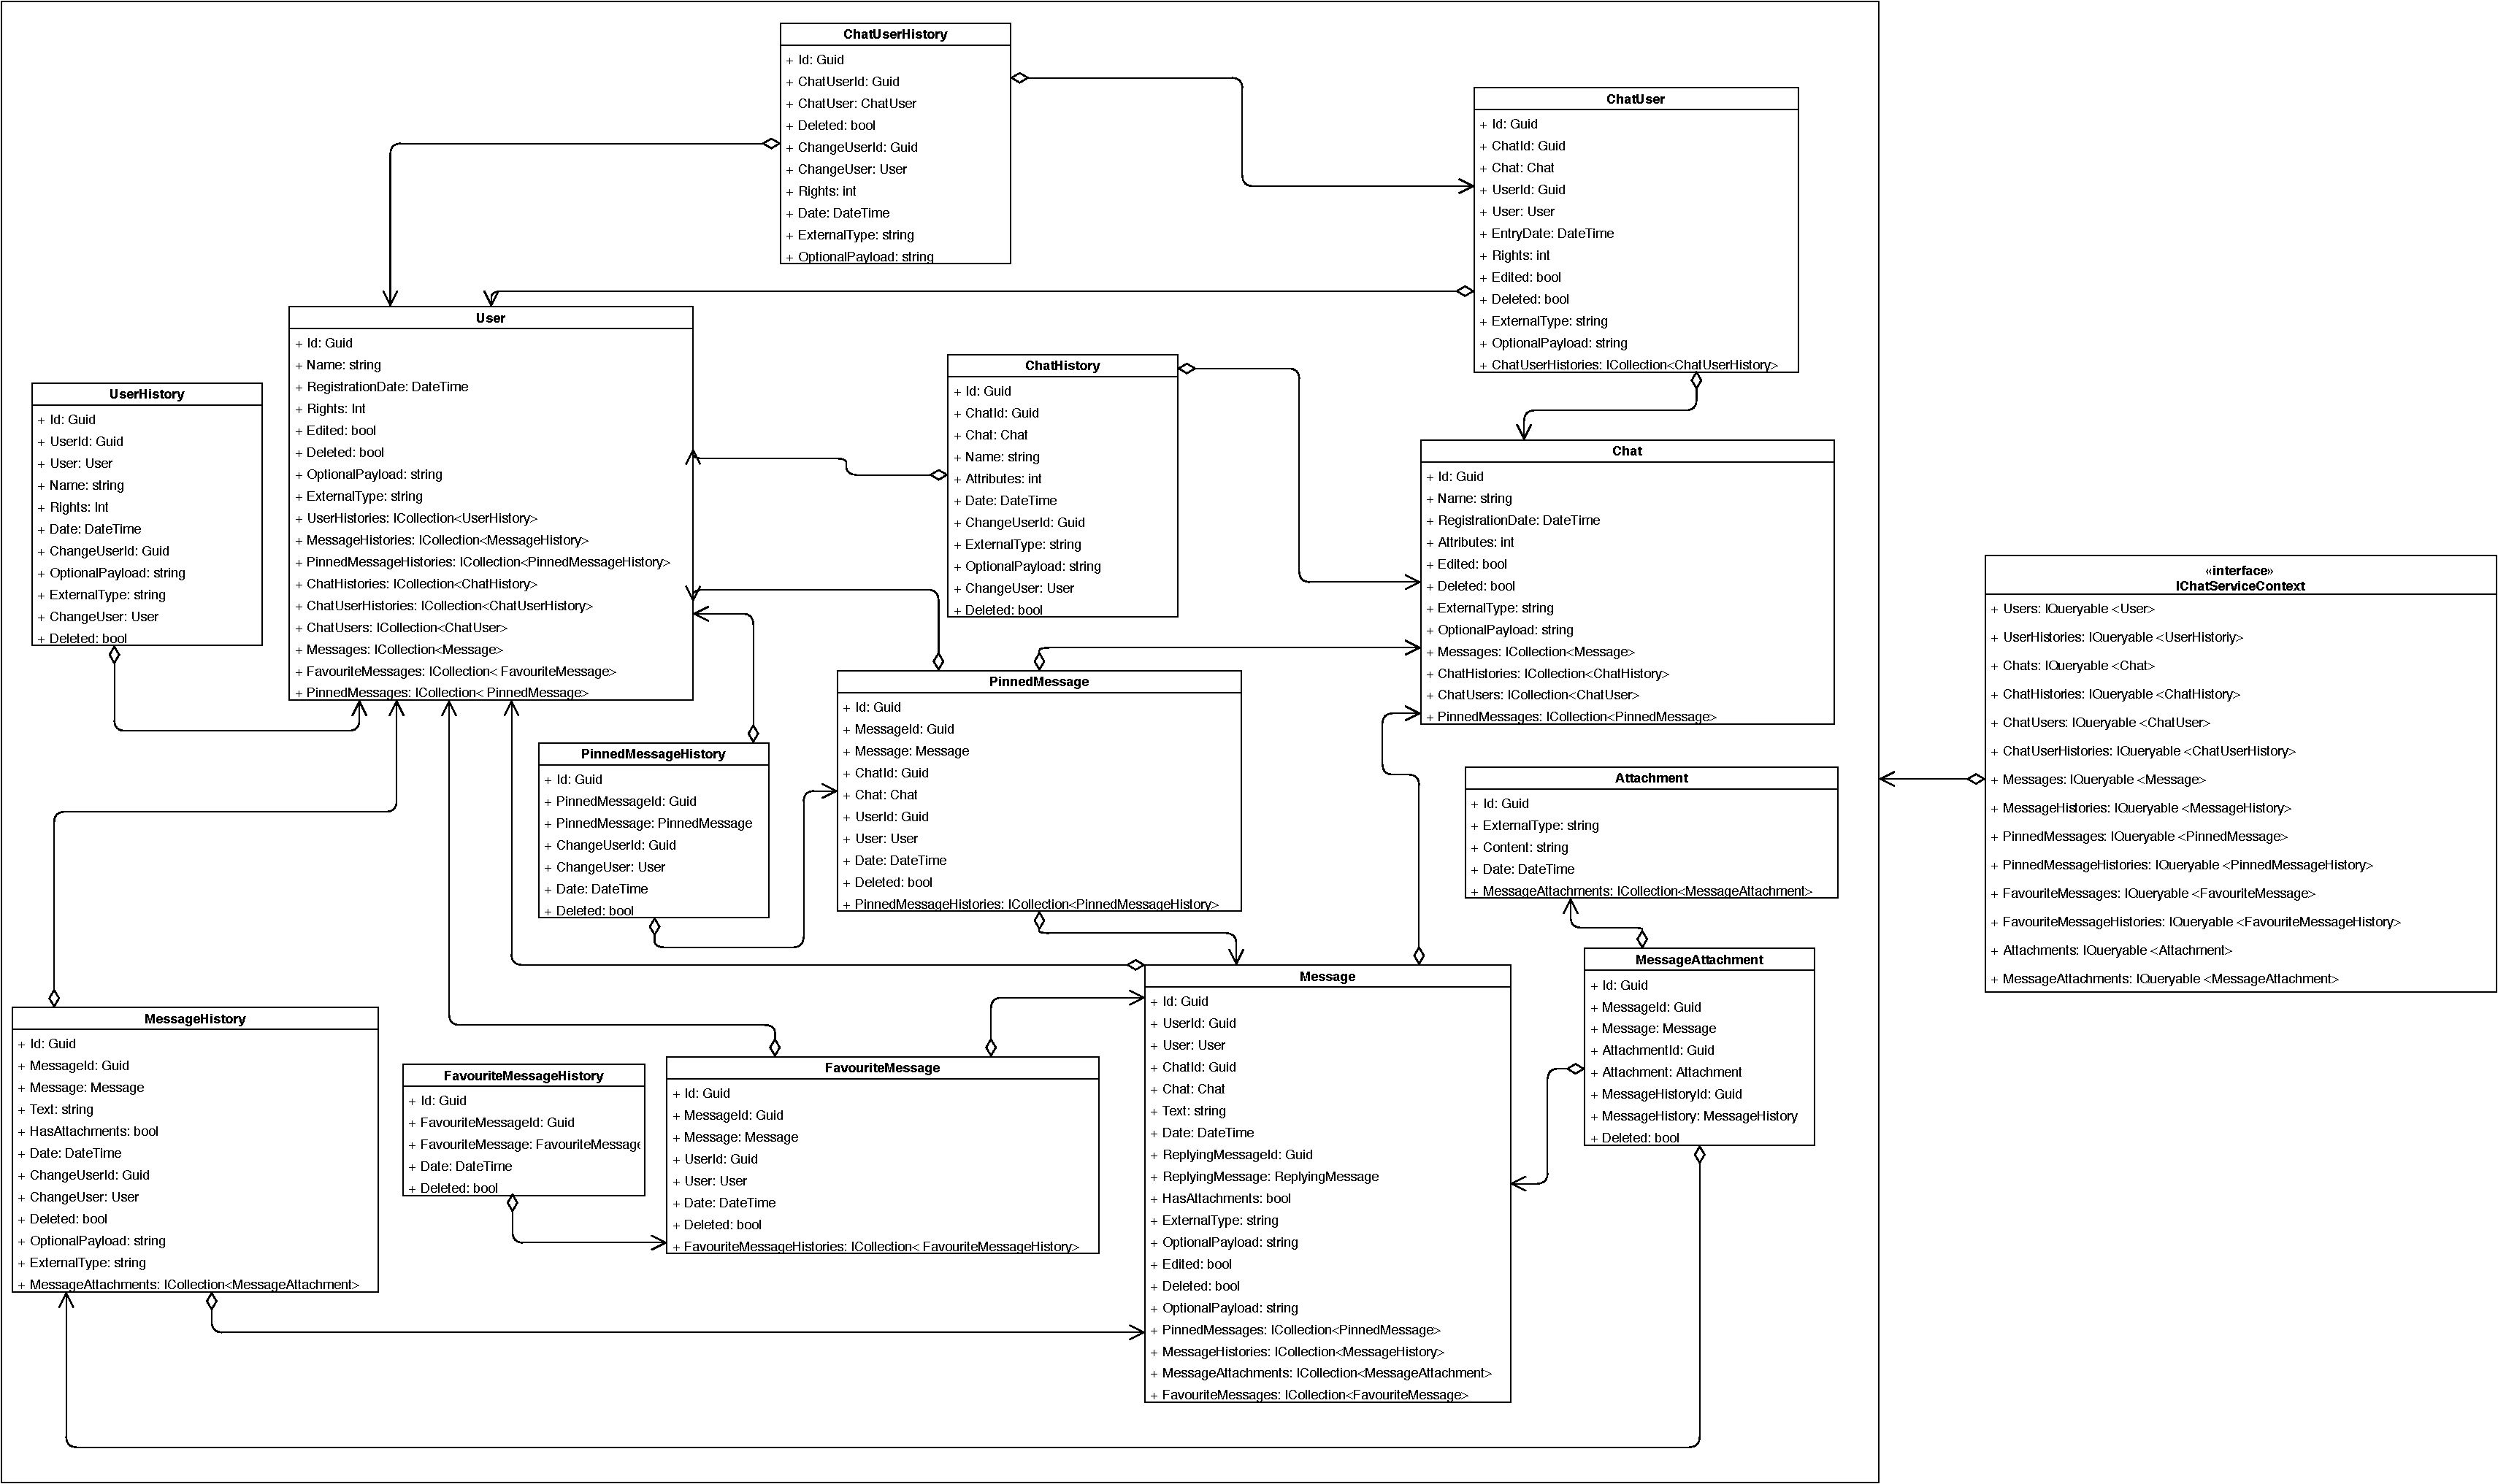
\includegraphics[scale=0.3]{databasemodels}
	\caption{UML-диаграмма классов компонента ChatService.Database.Models. }
	\label{img:databasemodels}
\end{figure}

На рисунке \ref{img:npgsqlcontext} представлена UML-диаграмма классов компонента ChatService.Database.NpgsqlContext. 

\begin{figure}[H]
	\centering
	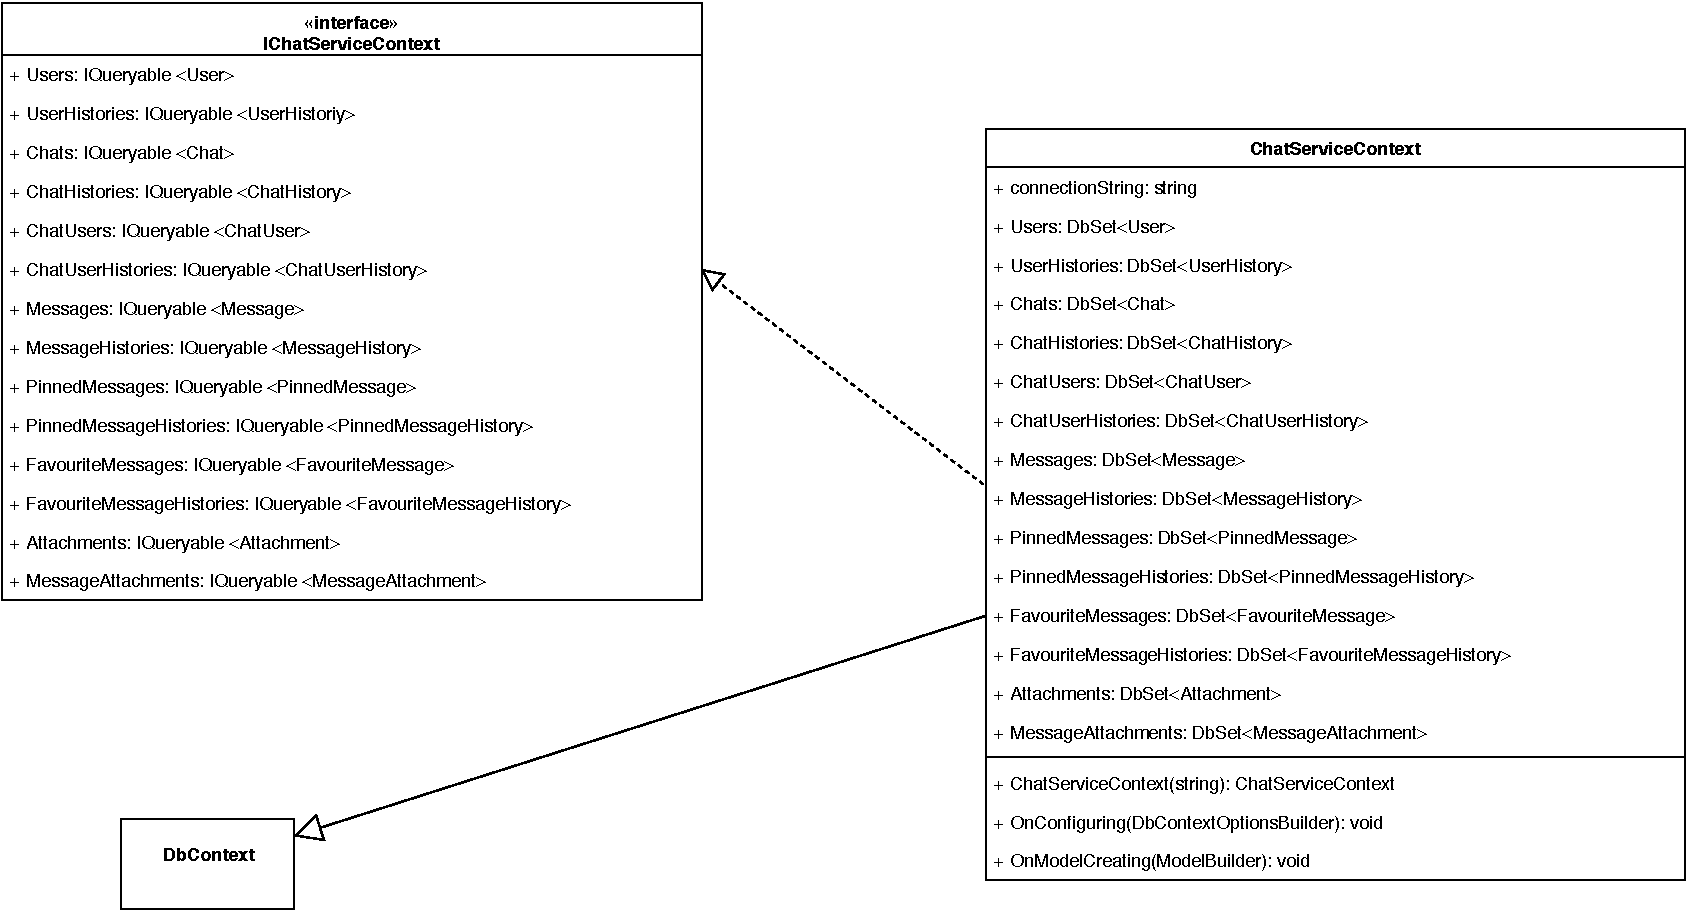
\includegraphics[scale=0.60]{npgsqlcontext}
	\caption{UML-диаграмма классов компонента ChatService.Database.NpgsqlContext. }
	\label{img:npgsqlcontext}
\end{figure}

На рисунке \ref{img:core} представлена UML-диаграмма классов компонента ChatService.Core. 

\begin{figure}[H]
	\centering
	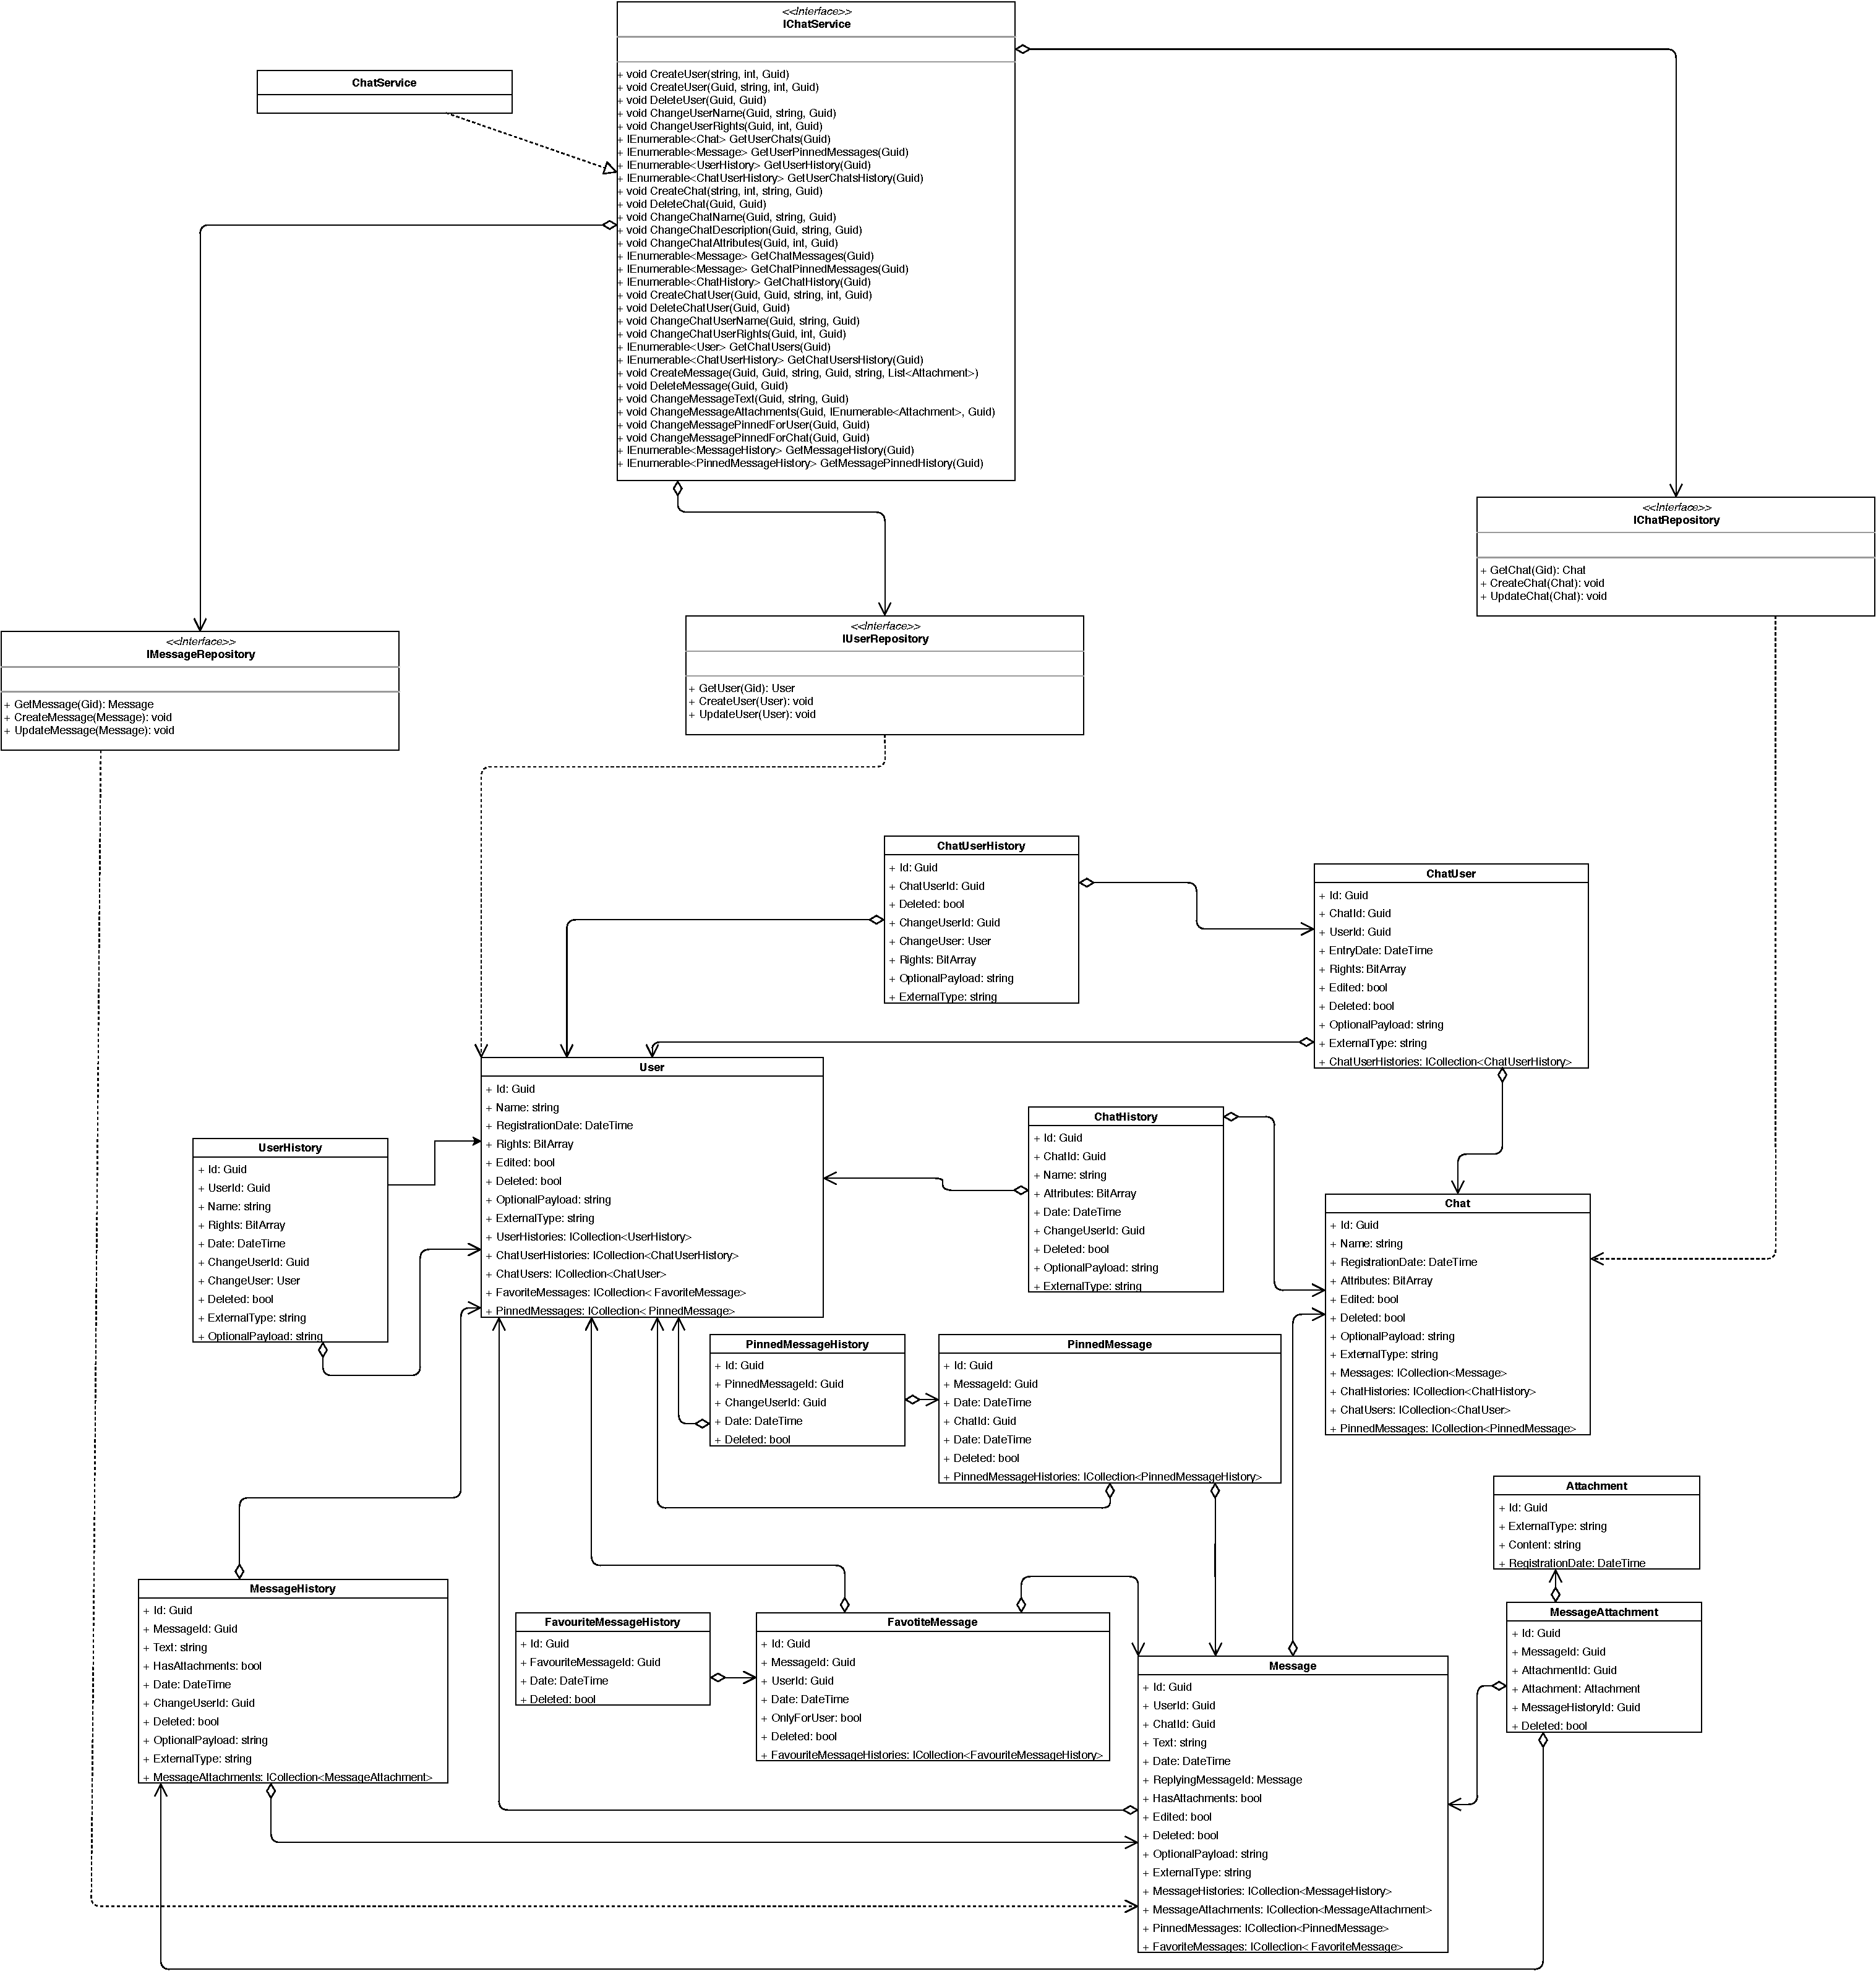
\includegraphics[scale=0.35]{core}
	\caption{UML-диаграмма классов компонента ChatService.Core. }
	\label{img:core}
\end{figure}

\textbf{Описание методов данного компонента:}
\begin{itemize}
\item void CreateUser(string name, int rights, Guid changeUserId) - добавление пользователя
\item void CreateUser(Guid userId, string name, int rights, Guid changeUserId) - добавление пользователя
\item void DeleteUser(Guid userId, Guid changeUserId) - удаление пользователя
\item void ChangeUserName(Guid userId, string newName, Guid changeUserId) - изменение имени пользователя
\item void ChangeUserRights(Guid userId, int newRights, Guid changeUserId) - изменение прав пользователя
\item IEnumerable<Chat> GetUserChats(Guid userId) - получение списка чатов пользователя
\item IEnumerable<Message> GetUserPinnedMessages(Guid userId) - получение списка избранных сообщений пользователя
\item IEnumerable<UserHistory> GetUserHistory(Guid userId) - получение всей истории пользователя
\item IEnumerable<ChatUserHistory> GetUserChatsHistory(Guid userId) - получение истории чатов пользователя
\item void CreateChat(string name, int attributes, string desciption, Guid changeUserId) - добавление чата
\item void DeleteChat(Guid chatId, Guid changeUserId) - удаление чата
\item void ChangeChatName(Guid chatId, string newName, Guid changeUserId) - изменение имени чата
\item void ChangeChatDescription(Guid chatId, string newDescription, Guid changeUserId) - изменение описания чата
\item void ChangeChatAttributes(Guid chatId, int newAttributes, Guid changeUserId) - изменение аттрибутов чата
\item IEnumerable<Message> GetChatMessages(Guid chatId) - получение сообщений чата
\item IEnumerable<Message> GetChatPinnedMessages(Guid chatId) - получение припиненных сообщений чата
\item IEnumerable<ChatHistory> GetChatHistory(Guid chatId) - получение истории чата
\item void CreateChatUser(Guid chatId, Guid userId, string name, int rights, Guid changeUserId) - добавление пользователя в чат
\item void DeleteChatUser(Guid chatUserId, Guid changeUserId) - удаление пользователя из чата
\item void ChangeChatUserName(Guid chatUserId, string newName, Guid changeUserId) - изменение имени пользователя чата
\item void ChangeChatUserRights(Guid chatUserId, int rights, Guid changeUserId) - изменение прав пользователя чата
\item IEnumerable<User> GetChatUsers(Guid chatId) - получение пользователей чата
\item IEnumerable<ChatUserHistory> GetChatUsersHistory(Guid chatId) - получение истории пользователей чата
\item void CreateMessage(Guid userId, Guid chatId, string text, Guid replyingMessageId, string type, List<Attachment> messageAttachments) - добавление сообщения
\item void DeleteMessage(Guid messageId, Guid changeUserId) - удаление сообщения
\item void ChangeMessageText(Guid messageId, string newText, Guid changeUserId) - изменение текста сообщения
\item void ChangeMessageAttachments(Guid messageId, IEnumerable<Attachment> newMessageAttchments, Guid changeUserId) - изменение вложений сообщения
\item void ChangeMessagePinnedForUser(Guid userId, Guid changeUserId) - припинивание/отпинивание сообщения для пользователя
\item void ChangeMessagePinnedForChat(Guid userId, Guid changeUserId) - припинивание/отпинивание сообщения для чата
\item IEnumerable<MessageHistory> GetMessageHistory(Guid messageId) - получение истории сообщения
\item IEnumerable<PinnedMessageHistory> GetMessagePinnedHistory(Guid messageId) - получение истории припинивания сообщения
\end{itemize}

\section{\textbf{Тестовое клиентское приложение }}

Реализовано с помощью 

Запуск приложения представлен на рисунке \ref{img:init}. 

\begin{figure}[H]
	\centering
	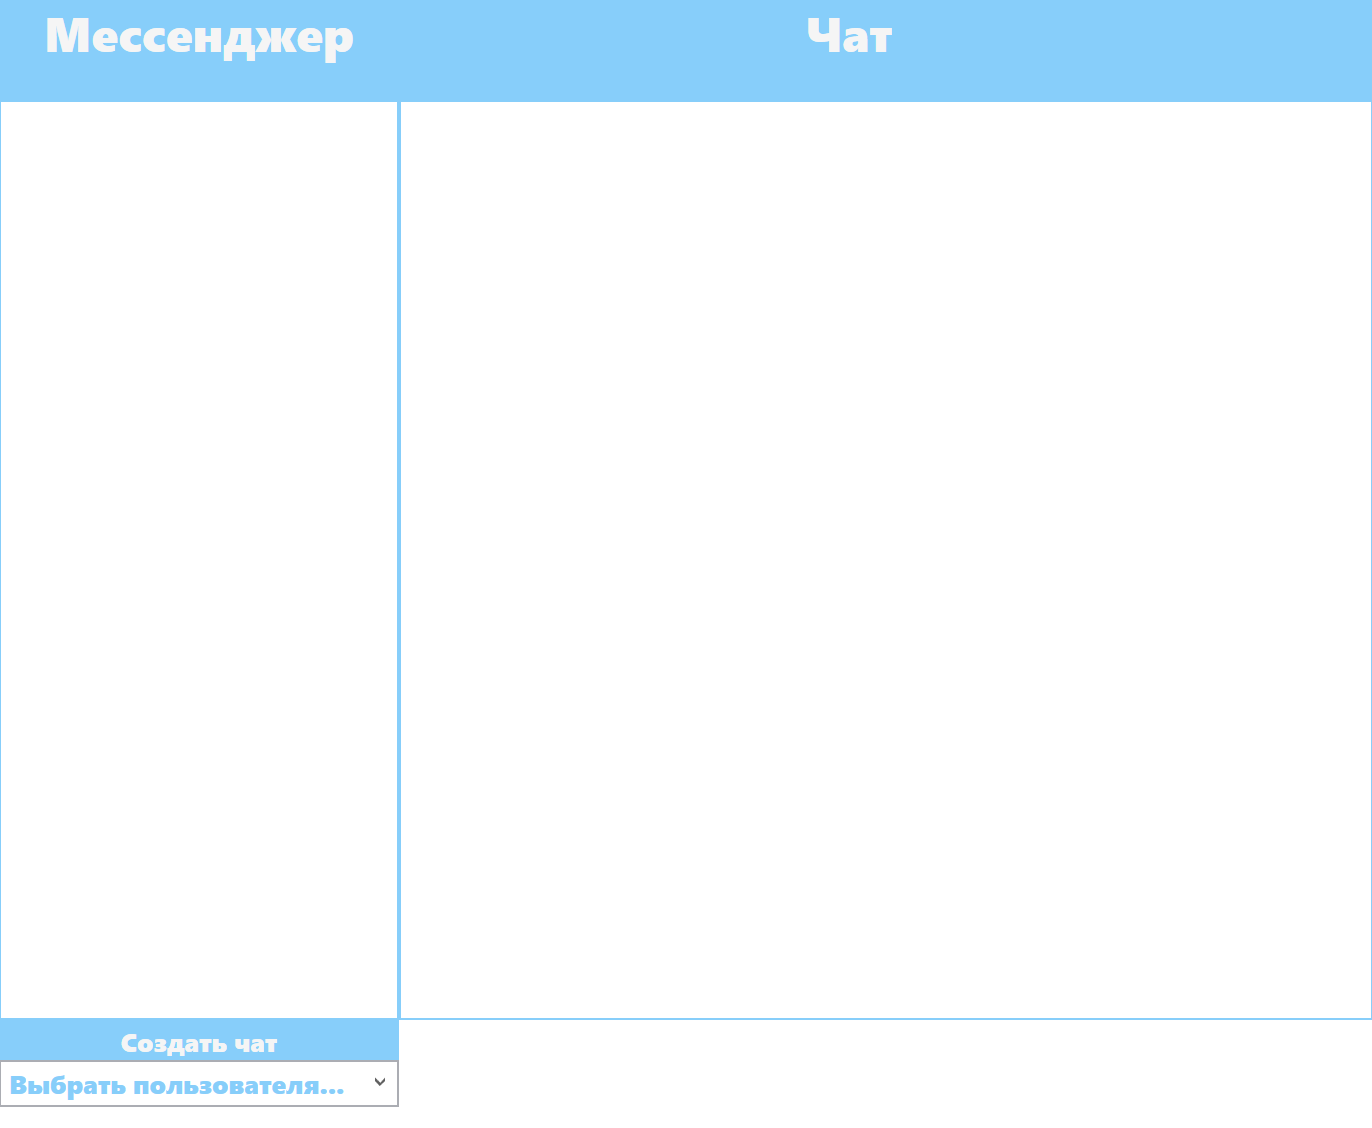
\includegraphics[scale=0.7]{init}
	\caption{Начальный экран приложения.  }
	\label{img:init}
\end{figure}

Далее можно выбрать текущего пользователя, от имени которого будут происходить дальнейшие действия, рисунок \ref{img:users}. 

\begin{figure}[H]
	\centering
	
\includegraphics[scale=1]{users}
	\caption{Выбор пользователя.  }
	\label{img:users}
\end{figure}

Далее можно выбрать чат, рисунок \ref{img:messenger}.

Сообщения чата обновляются каждую секунду. Отправить сообщение можно либо по нажатию на кнопку, либо по нажатию на клавишу "Enter". Отправка пустого сообщения невозможна. 

\begin{figure}[H]
	\centering
	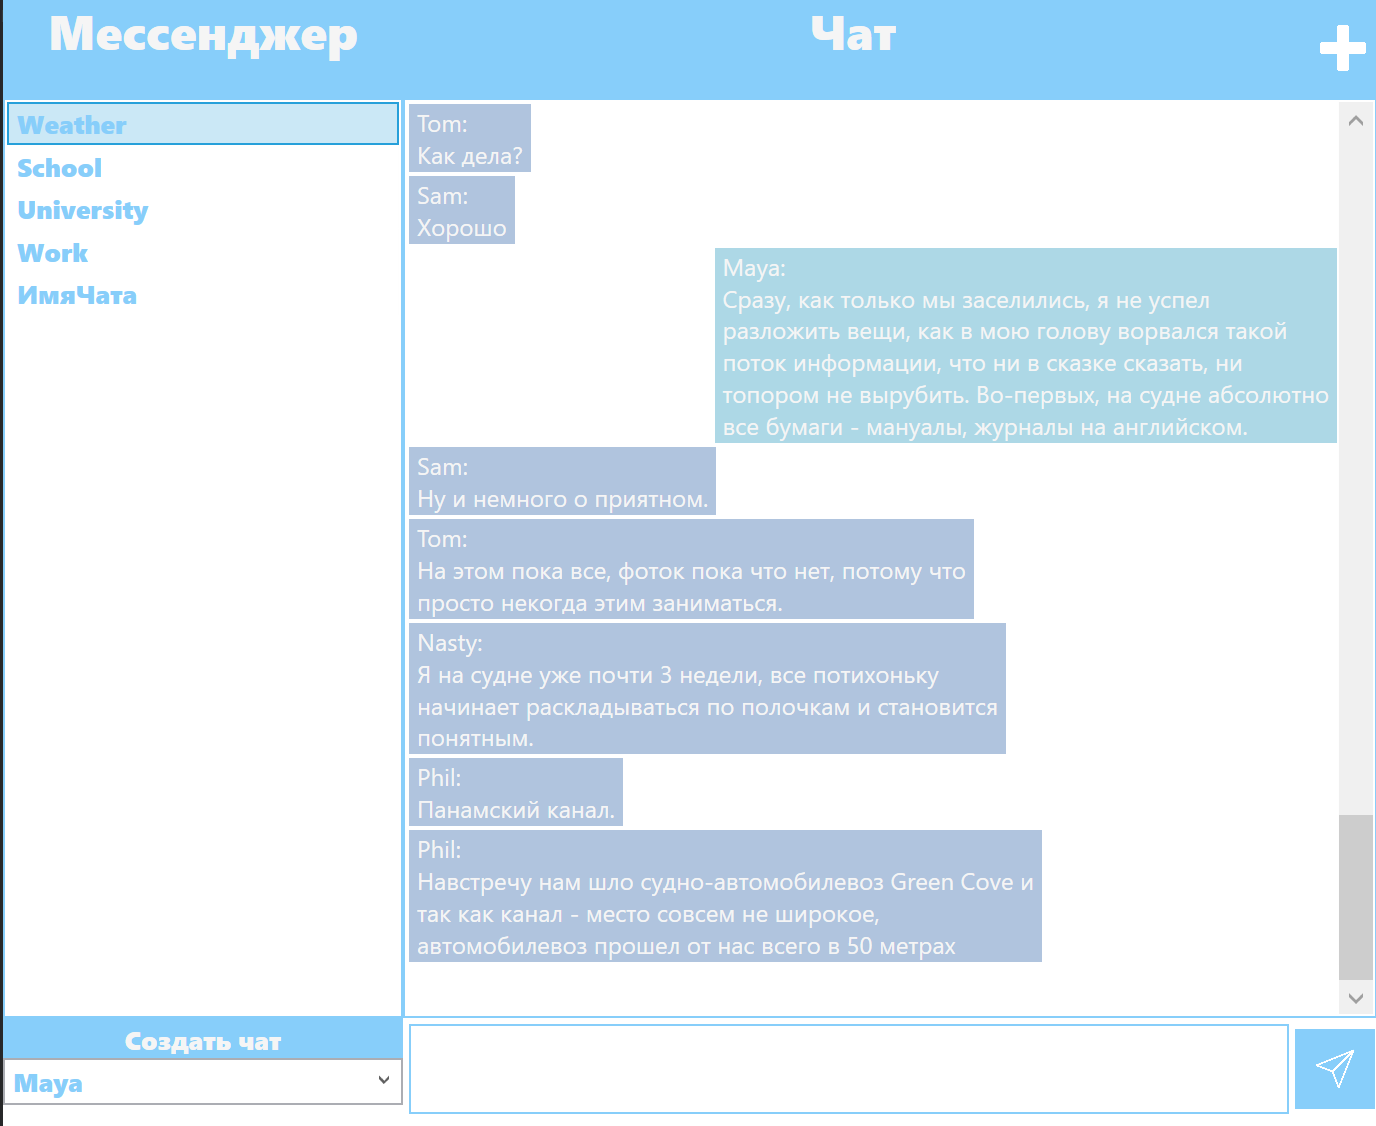
\includegraphics[scale=0.7]{messenger}
	\caption{Выбор чата, отображение сообщений.  }
	\label{img:messenger}
\end{figure}

Есть возможность из интерфейса создать новый чат (\ref{img:addchat}), нового пользователя \ref{img:adduser} или добавить пользователей (одного или нескольких) в уже существующий чат \ref{img:addchatuser}. 

\begin{figure}[H]
	\centering
	
\includegraphics[scale=1]{addchat}
	\caption{Создание чата.  }
	\label{img:addchat}
\end{figure}

\begin{figure}[H]
	\centering
	
\includegraphics[scale=1]{adduser}
	\caption{Создание пользователя.  }
	\label{img:adduser}
\end{figure}

\begin{figure}[H]
	\centering
	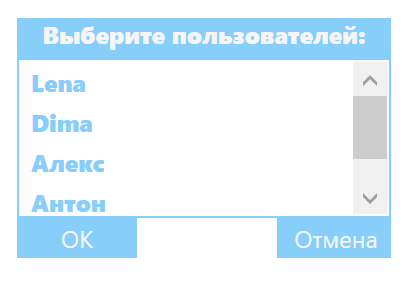
\includegraphics[scale=1]{addchatuser}
	\caption{Добавление пользователя/пользователей чат.  }
	\label{img:addchatuser}
\end{figure}

\section{\textbf{Администрирование БД}}

С использованием pgAdmin (программное обеспечение, предоставляющее графический интерфейс для работы с базой данных) было проверено корректное создание базы данных с необходимыми ключами. 

На рисунке \ref{img:tables} показано существование таблицы в БД. 

\begin{figure}[H]
	\centering
	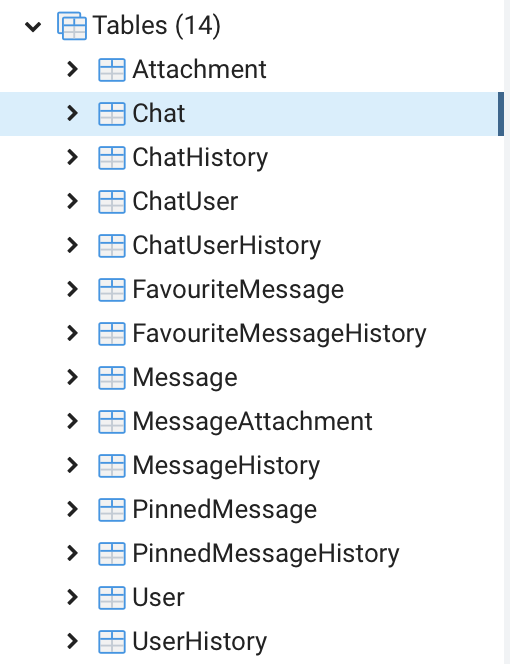
\includegraphics[scale=1]{tables}
	\caption{Таблицы базы данных.  }
	\label{img:tables}
\end{figure}

На рисунке \ref{img:chattable} показан пример корректности ключей для таблицы чатов.  

\begin{figure}[H]
	\centering
	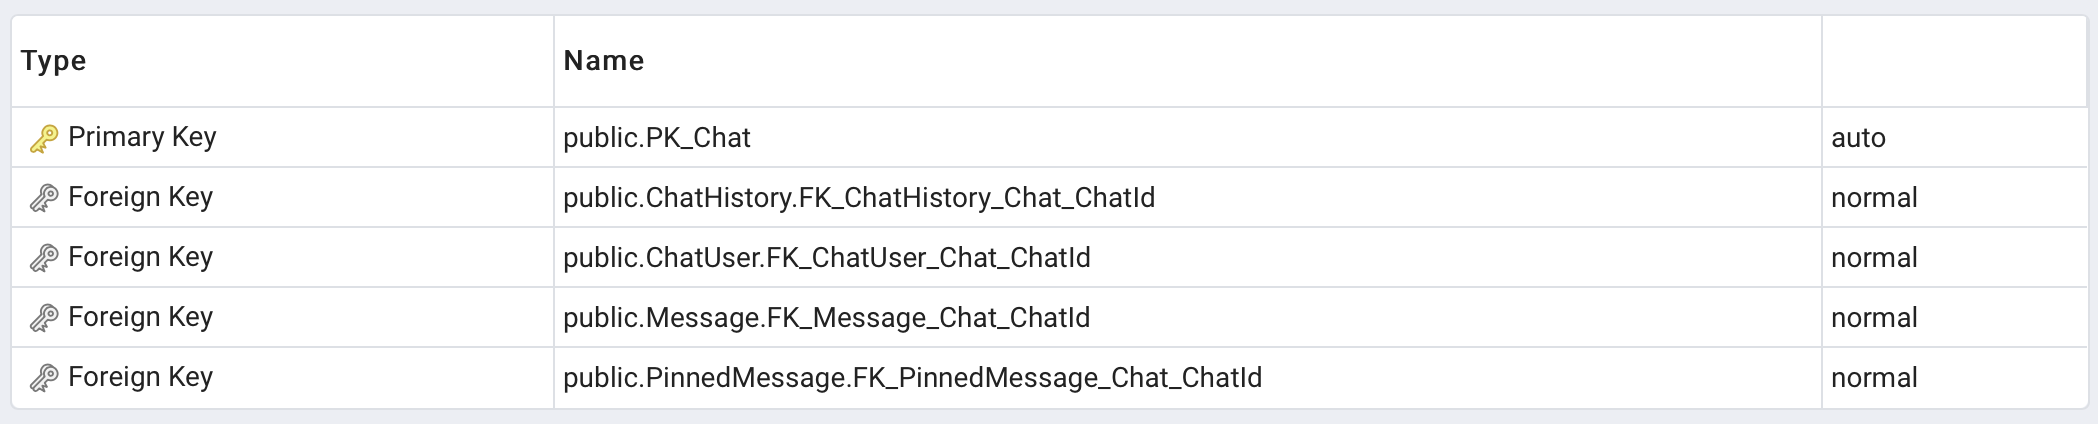
\includegraphics[scale=0.45]{chattable}
	\caption{Ключи таблицы чатов. }
	\label{img:chattable}
\end{figure}


\section{\textbf{Вывод}}

Реализовано спроектированное ПО, представлены результаты. 


\backmatter %% Здесь заканчивается нумерованная часть документа и начинаются ссылки и
            
\Conclusion % заключение к отчёту

\hfill

В результате проделанной работы выполнены следующие задачи:
\begin{enumerate}
		\item проанализированы существующие решения; 
		\item спроектирован микросервис мессенджера;
		\item реализовано спроектированное ПО. 
	\end{enumerate}
	
Достигнута цель проекта -- реализация микросервиса универсального мессенджера. 

Реализован микросервис на языке программирования C$\#$ с использованием платформы ASP.NET Core и технологии Entity Framework Core. %% заключение


% % Список литературы при помощи BibTeX
% Юзать так:
%
% pdflatex rpz
% bibtex rpz
% pdflatex rpz

\bibliographystyle{ugost2008}
\bibliography{rpz}
\nocite{*}
%%% Local Variables: 
%%% mode: latex
%%% TeX-master: "rpz"
%%% End: 


\appendix   % Тут идут приложения

%\chapter{Картинки}


%%% Local Variables: 
%%% mode: latex
%%% TeX-master: "rpz"
%%% End: 


\end{document}

%%% Local Variables:
%%% mode: latex
%%% TeX-master: t
%%% End:
